\begin{appendices}

\chapter{Cut and Match Results}
\label{App:CutAndMatchingResults}

\newpage 

\section{Cut Results}
\begin{figure}[H]
  \centering
  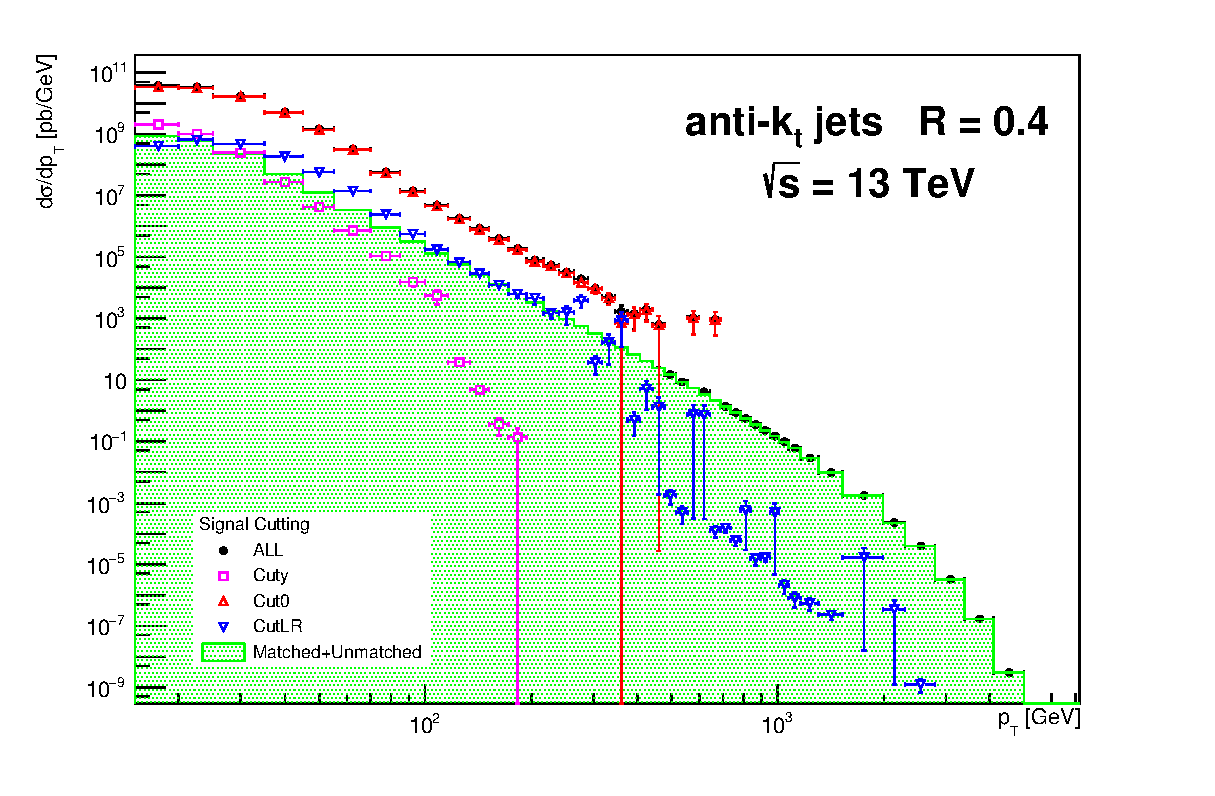
\includegraphics[width=0.9\textwidth]{Chapter3/SignalCutting.eps}
  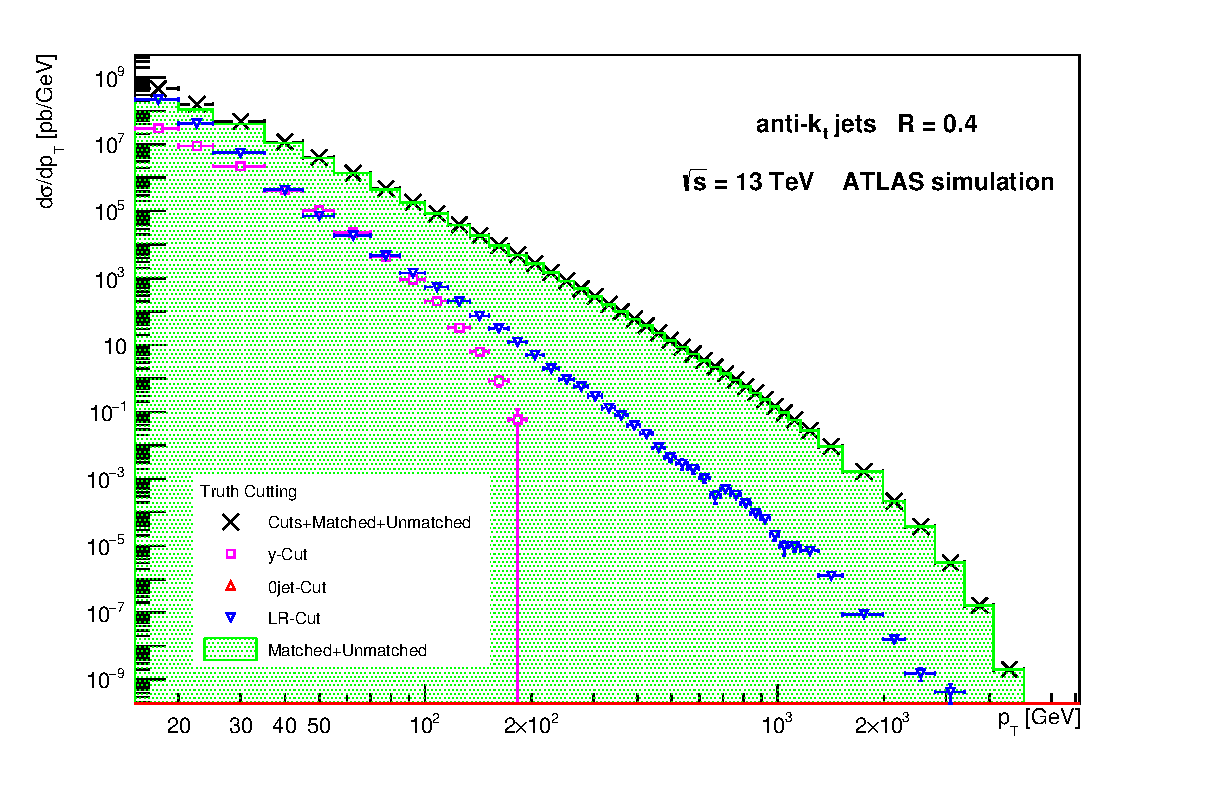
\includegraphics[width=0.9\textwidth]{Chapter3/TruthCutting.eps}
  \caption{Impact of 4 cuts defined in Section \ref{SubSec:JetCuts} on
  differential cross section in $\pt$ of signal jets (top) and truth jets
  (bottom). Black dots represent the original uncutted spectrum, green area then
  these jets, which survived all four cutoffs.}
  \label{fig:Cutting}
\end{figure}

\section{Match Results}
\begin{figure}[H]
  \centering
  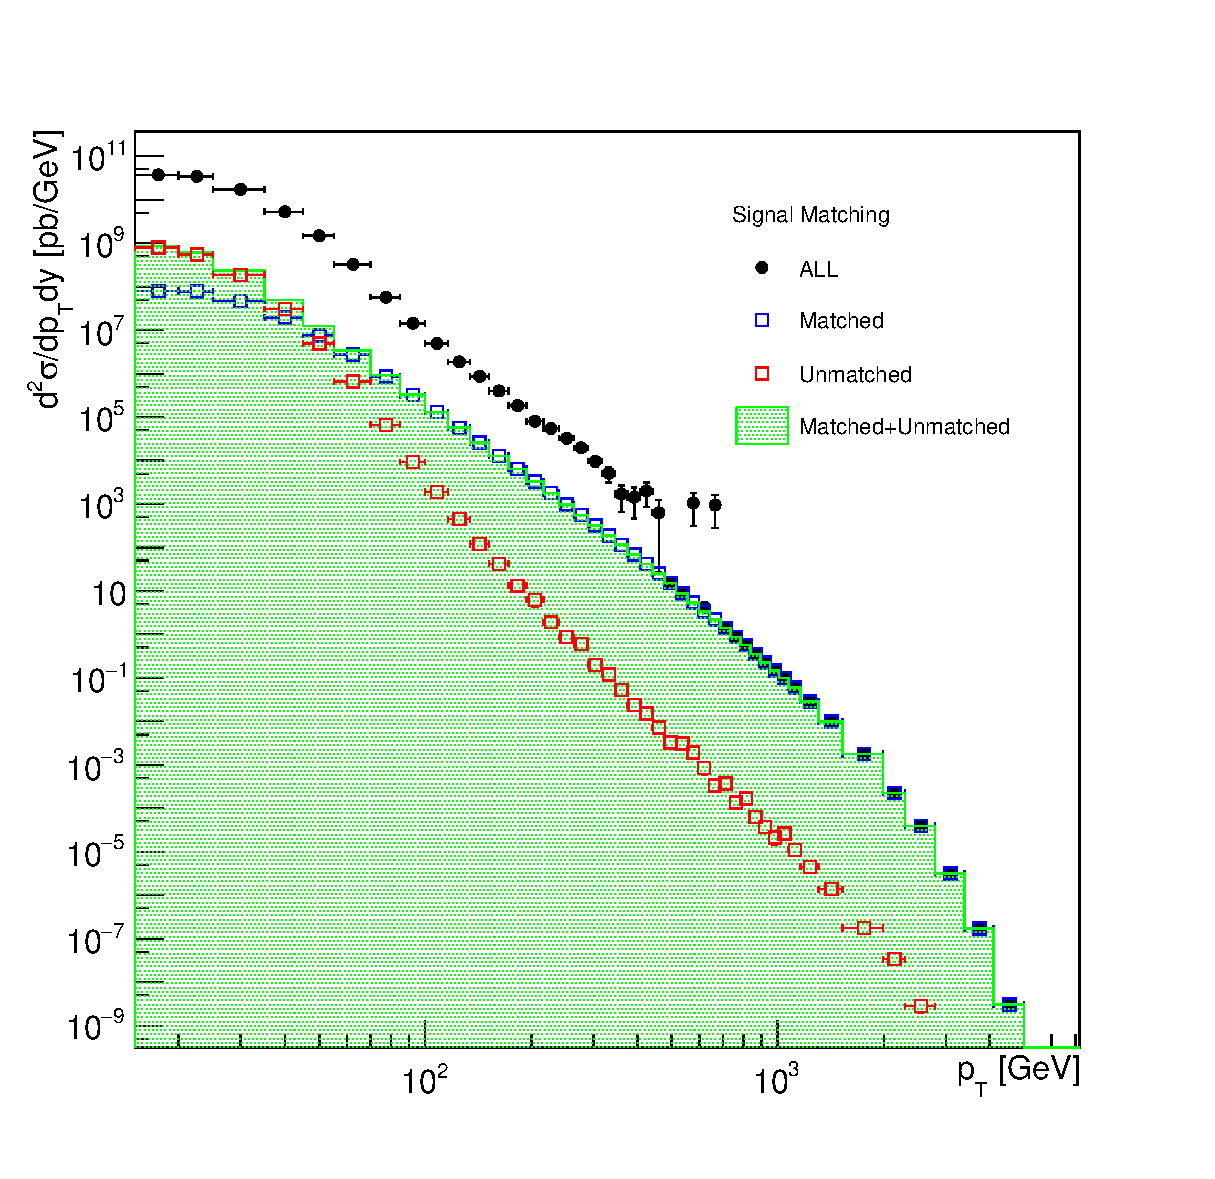
\includegraphics[width=0.9\textwidth]{Chapter3/SignalMatching.eps}
  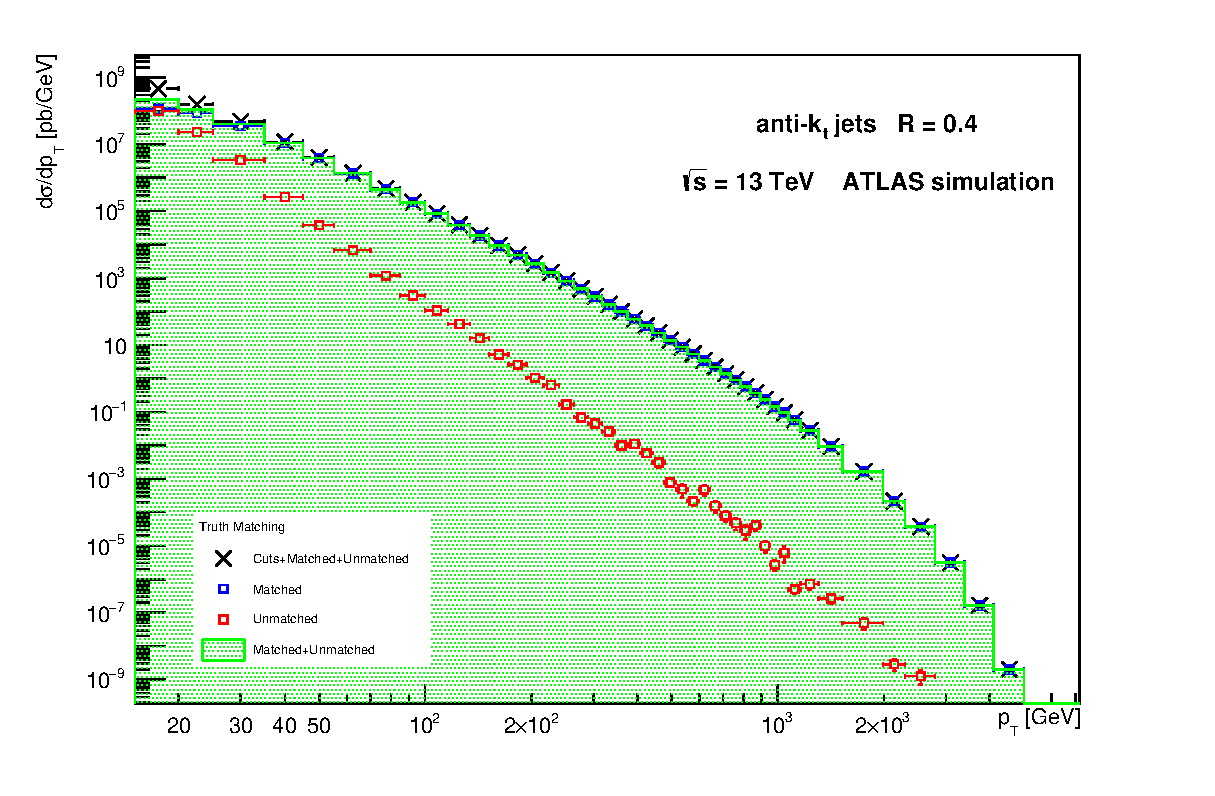
\includegraphics[width=0.9\textwidth]{Chapter3/TruthMatching.eps}
  \caption{Results of matching procedure described in Section
  \ref{SubSec:JetMatching} demonstrated on differential cross section in $\pt$ of
  signal (top) and truth (bottom) jets. Black dots represent the original
  uncutted spectrum. The contribution of matched and unmatched jets to
  green area representing all jets which survived cutoffs is shown.}
  \label{fig:Matching}
\end{figure}

\section{Truth and Reco $\pt$ Spectra}
\begin{figure}[H]
  \centering
  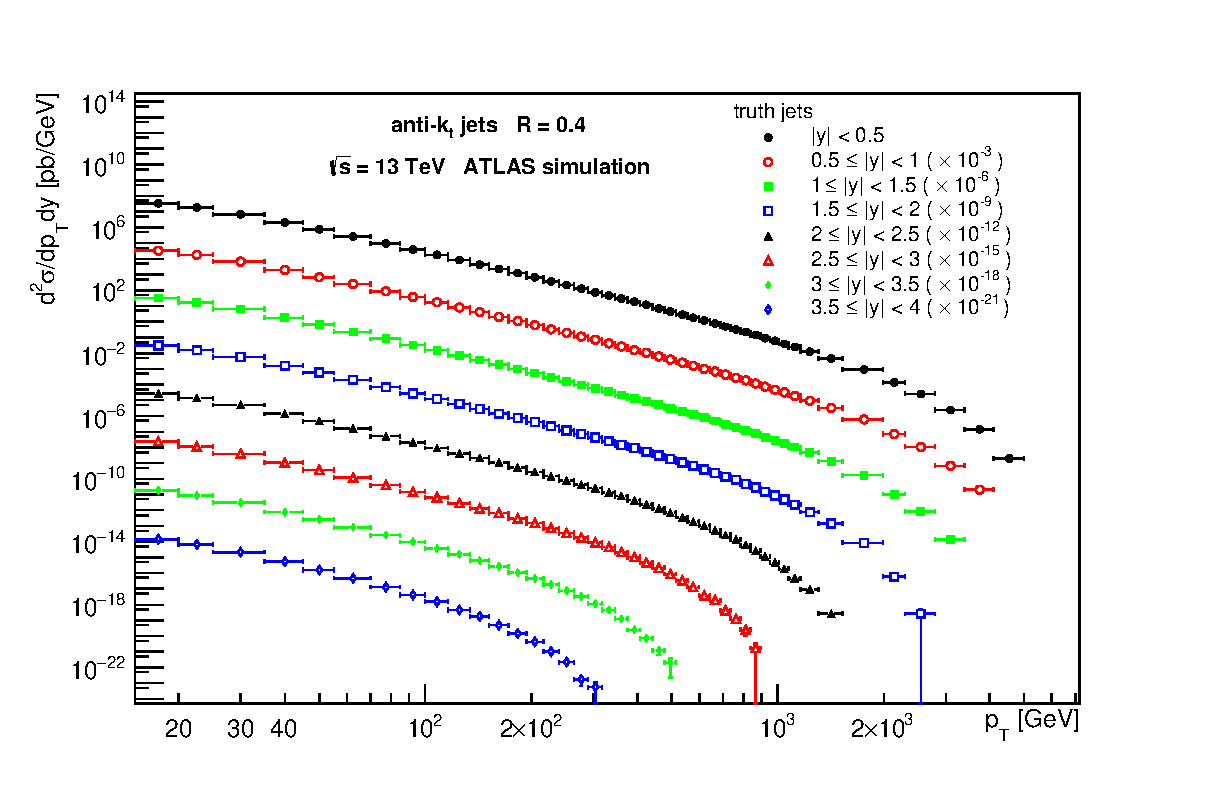
\includegraphics[width=\textwidth]{Chapter3/ptTruthAllRapidityBins.eps}
  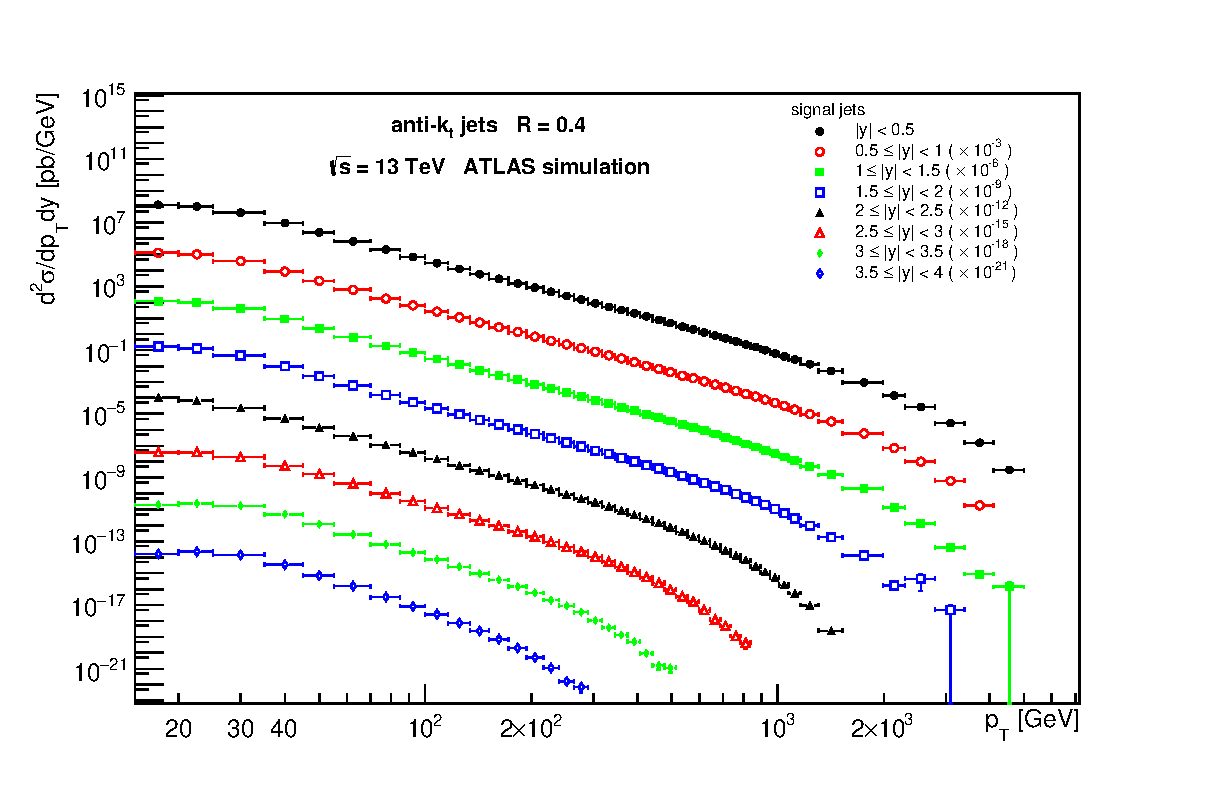
\includegraphics[width=\textwidth]{Chapter3/ptSignalAllRapidityBins.eps}
\end{figure}


\begin{landscape} 
\begin{table}
  \small
  \centering
  \begin{tabular}{|c|c|>{\bfseries}c|c|c|c|c|c|c|c|c|}
    \hline
     \multicolumn{2}{|c|}{\# jets}  & ALL      & JZ0W     & JZ1W     & JZ2W     & JZ3W     & JZ4W     & JZ5W     & JZ6W     & JZ7W     \\
    \hline                                                              
    \hline                                                              
     \multicolumn{2}{|c|}{Signal}                               & 1.09e+08 & 3.11e+07 & 3.59e+07 & 6.67e+06 & 7.07e+06 & 6.28e+06 & 7.29e+06 & 7.13e+06 & 7.11e+06 \\
    \hline                                                                                          
     \multicolumn{2}{|c|}{Truth}                                & 7.28e+07 & 3.04e+06 & 3.00e+07 & 6.17e+06 & 6.91e+06 & 6.20e+06 & 6.98e+06 & 6.53e+06 & 6.25e+06 \\
    \hline                                                                                      
    \hline                                                                                      
    \multirow{4}{*}{CutPt}          & \multirow{2}{*}{Signal}   & 9.36e+06 & 3.74e+06 & 3.13e+06 & 6.50e+05 & 5.87e+05 & 4.76e+05 & 5.48e+05 & 5.52e+05 & 5.63e+05 \\
                                    &                           & 8.6 \%   & 12.0 \%  & 8.7 \%   & 9.7 \%   & 8.3 \%   & 7.6 \%   & 7.5 \%   & 7.7 \%   & 7.9 \%   \\
    \cline{2-11}                                                                                
                                    & \multirow{2}{*}{Truth}    & 4.70e+07 & 3.00e+06 & 2.20e+07 & 3.86e+06 & 4.00e+06 & 3.42e+06 & 3.74e+06 & 3.43e+06 & 3.23e+06 \\
                                    &                           & 64.6 \%  & 98.7 \%  & 73.1 \%  & 62.6 \%  & 57.8 \%  & 55.1 \%  & 53.6 \%  & 52.5 \%  & 51.6 \%  \\
    \hline                                                                                      
    \hline                                                                                      
    \multirow{4}{*}{Cuty}           & \multirow{2}{*}{Signal}   & 3.43e+06 & 1.19e+06 & 1.29e+06 & 1.42e+05 & 1.28e+05 & 1.03e+05 & 1.16e+05 & 1.10e+05 & 1.08e+05 \\
                                    &                           & 3.1 \%   & 3.8 \%   & 3.6 \%   & 2.1 \%   & 1.8 \%   & 1.6 \%   & 1.6 \%   & 1.5 \%   & 1.5 \%   \\
    \cline{2-11}                                                                                    
                                    & \multirow{2}{*}{Truth}    & 5.06e+05 & 3.04e+03 & 3.19e+05 & 4.54e+04 & 3.79e+04 & 2.88e+04 & 2.78e+04 & 2.22e+04 & 1.83e+04 \\
                                    &                           & 0.7 \%   & 0.1 \%   & 1.1 \%   & 0.7 \%   & 0.5 \%   & 0.5 \%   & 0.4 \%   & 0.3 \%   & 0.3 \%   \\
    \hline                                                                                      
    \hline                                                                                      
    \multirow{4}{*}{Cut0jet}        & \multirow{2}{*}{Signal}   & 2.64e+07 & 2.59e+07 & 5.70e+05 & 0.00e+00 & 0.00e+00 & 0.00e+00 & 0.00e+00 & 0.00e+00 & 0.00e+00 \\
                                    &                           & 24.2 \%  & 83.2 \%  & 1.6 \%   & 0.0 \%   & 0.0 \%   & 0.0 \%   & 0.0 \%   & 0.0 \%   & 0.0 \%   \\
    \cline{2-11}                                                                                    
                                    & \multirow{2}{*}{Truth}    & 0.00e+00 & 0.00e+00 & 0.00e+00 & 0.00e+00 & 0.00e+00 & 0.00e+00 & 0.00e+00 & 0.00e+00 & 0.00e+00 \\
                                    &                           & 0.0 \%   & 0.0 \%   & 0.0 \%   & 0.0 \%   & 0.0 \%   & 0.0 \%   & 0.0 \%   & 0.0 \%   & 0.0 \%   \\
    \hline                                                                                      
    \hline                                                                                      
    \multirow{4}{*}{CutLR}          & \multirow{2}{*}{Signal}   & 4.09e+06 & 2.38e+05 & 3.82e+06 & 2.99e+04 & 7.07e+03 & 2.33e+03 & 1.63e+03 & 7.14e+02 & 6.31e+02 \\
                                    &                           & 3.7 \%   & 0.8 \%   & 10.6 \%  & 0.4 \%   & 0.1 \%   & 0.0 \%   & 0.0 \%   & 0.0 \%   & 0.0 \%   \\
    \cline{2-11}                                                                                    
                                    & \multirow{2}{*}{Truth}    & 5.40e+05 & 2.19e+04 & 4.96e+05 & 1.82e+04 & 4.45e+03 & 1.33e+03 & 9.03e+02 & 4.37e+02 & 2.78e+02 \\
                                    &                           & 0.7 \%   & 0.7 \%   & 1.7 \%   & 0.3 \%   & 0.1 \%   & 0.0 \%   & 0.0 \%   & 0.0 \%   & 0.0 \%   \\
    \hline                                                                                      
    \hline                                                                                      
    \multirow{4}{*}{Matched}        & \multirow{2}{*}{Signal}   & 2.17e+07 & 7.62e+03 & 6.03e+06 & 1.95e+06 & 2.54e+06 & 2.46e+06 & 2.88e+06 & 2.78e+06 & 2.72e+06 \\
                                    &                           & 19.8 \%  & 0.0 \%   & 16.8 \%  & 29.3 \%  & 36.0 \%  & 39.1 \%  & 39.5 \%  & 38.9 \%  & 38.2 \%  \\
    \cline{2-11}                                                                                    
                                    & \multirow{2}{*}{Truth}    & 2.17e+07 & 7.62e+03 & 6.03e+06 & 1.95e+06 & 2.54e+06 & 2.46e+06 & 2.88e+06 & 2.78e+06 & 2.72e+06 \\
                                    &                           & 29.8 \%  & 0.3 \%   & 20.1 \%  & 31.7 \%  & 36.8 \%  & 39.6 \%  & 41.3 \%  & 42.5 \%  & 43.5 \%  \\
    \hline                                                                                      
    \hline                                                                                      
    \multirow{4}{*}{Unmatched}      & \multirow{2}{*}{Signal}   & 4.42e+07 & 5.36e+04 & 2.10e+07 & 3.89e+06 & 3.81e+06 & 3.24e+06 & 3.75e+06 & 3.69e+06 & 3.72e+06 \\
                                    &                           & 40.5 \%  & 0.2 \%   & 58.6 \%  & 58.4 \%  & 53.8 \%  & 51.6 \%  & 51.4 \%  & 51.8 \%  & 52.3 \%  \\
    \cline{2-11}                                                                                    
                                    & \multirow{2}{*}{Truth}    & 3.07e+06 & 6.18e+03 & 1.25e+06 & 2.89e+05 & 3.29e+05 & 2.95e+05 & 3.29e+05 & 3.03e+05 & 2.88e+05 \\
                                    &                           & 4.2 \%   & 0.2 \%   & 4.2 \%   & 4.7 \%   & 4.8 \%   & 4.8 \%   & 4.7 \%   & 4.6 \%   & 4.6 \%   \\
    \hline
  \end{tabular}
  \caption{Statistics for matching and cutting procedures described in Sections
    \ref{SubSec:JetCuts} and \ref{SubSec:JetMatching} displayed for all jets and for
    individual JZXW samples defined in Table \ref{tab:JZXW}. At the top, there is
    number of initial signal and truth jets respectively. For each cut, there is
    shown the number of jets, which were killed by it, and their relative number
    according to the original number of signal or truth jets respectively.
    Last two lines show the statistics of matching procedure including number of
    jets which were (un)matched.}
  \label{tab:CutAndMatchingEfficiency}
\end{table} 
\end{landscape}

\chapter{Unfolding}
\label{App:UnfoldingResults}

\section{Matching Efficiency}

\begin{center}
\begin{figure}[H]
  \centering
  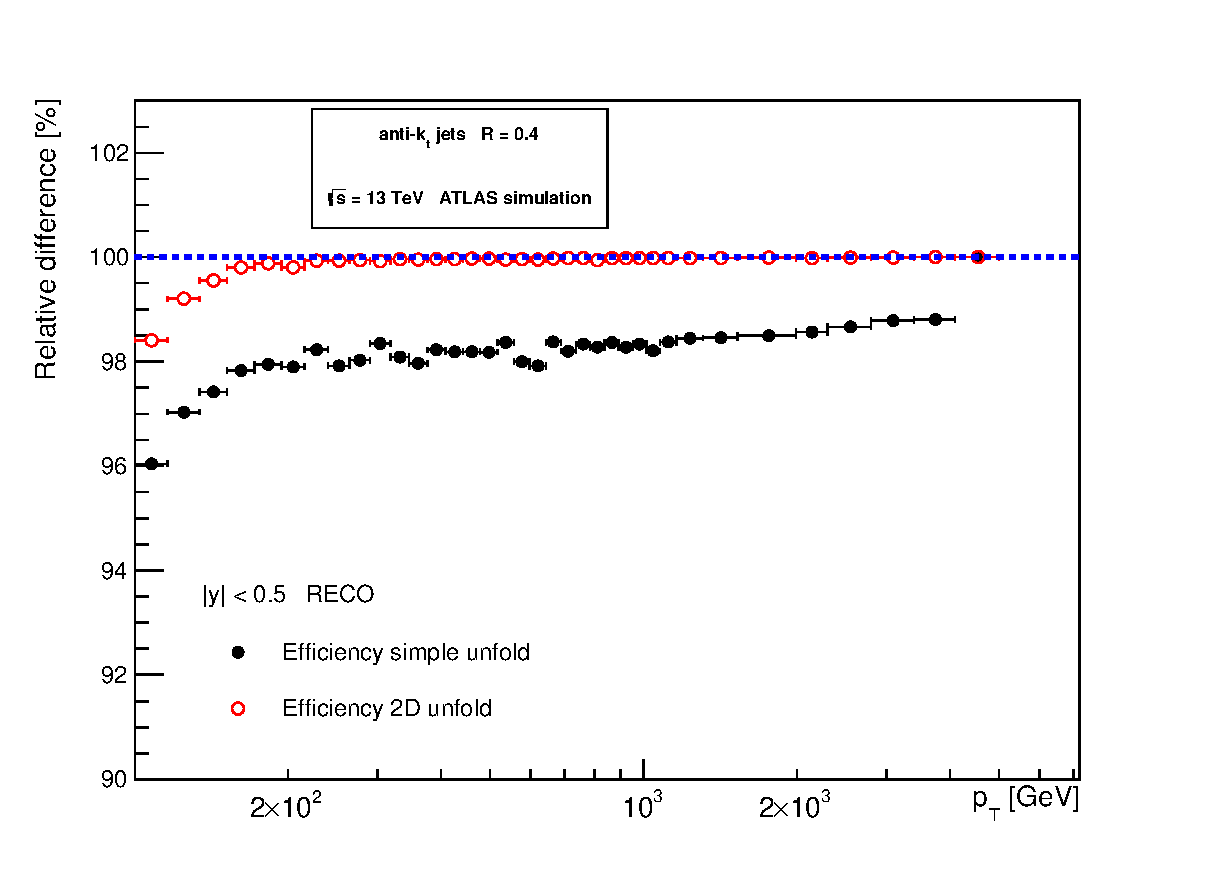
\includegraphics[width=0.49\textwidth]{{Chapter3/MatchEffSimpe2DSignal|abs(y)|0-0.5Compare}.eps}
  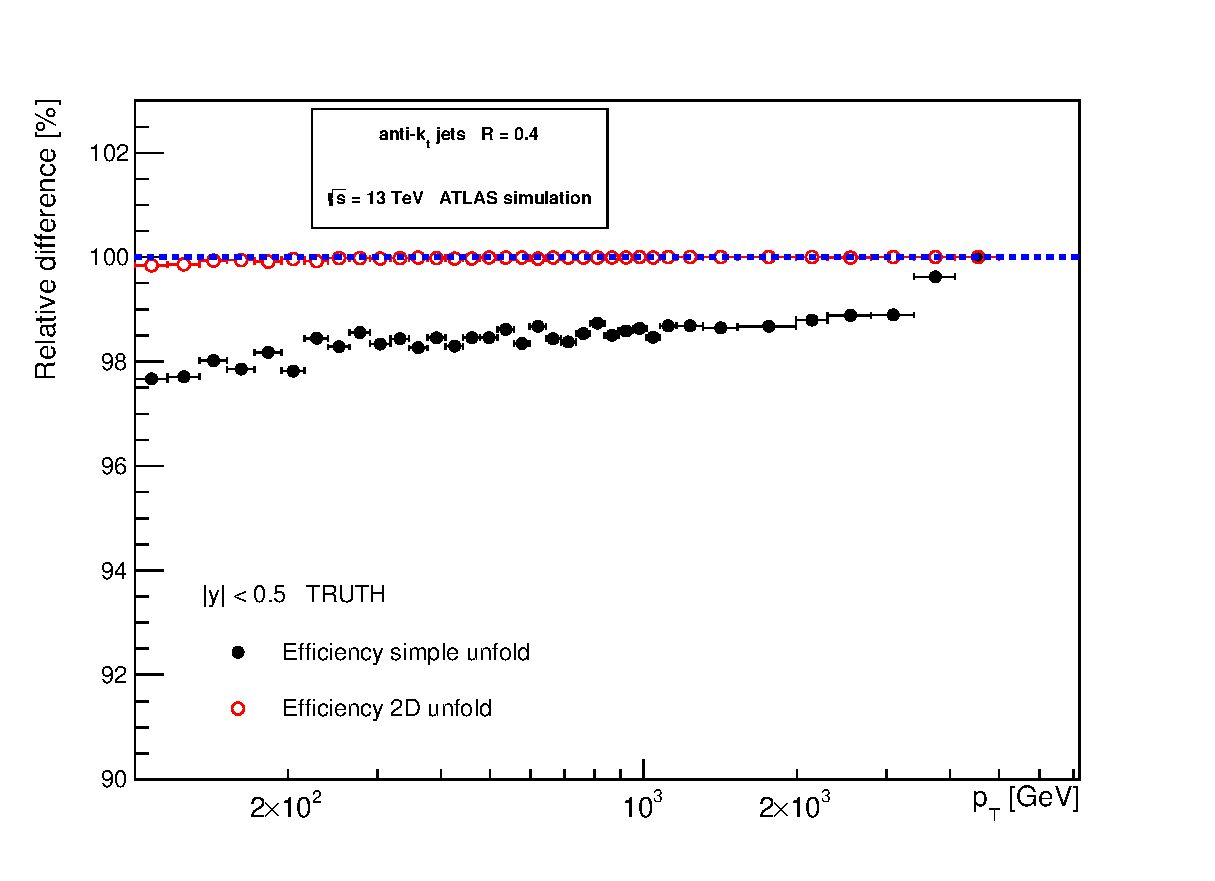
\includegraphics[width=0.49\textwidth]{{Chapter3/MatchEffSimpe2DTruth|abs(y)|0-0.5Compare}.eps}
  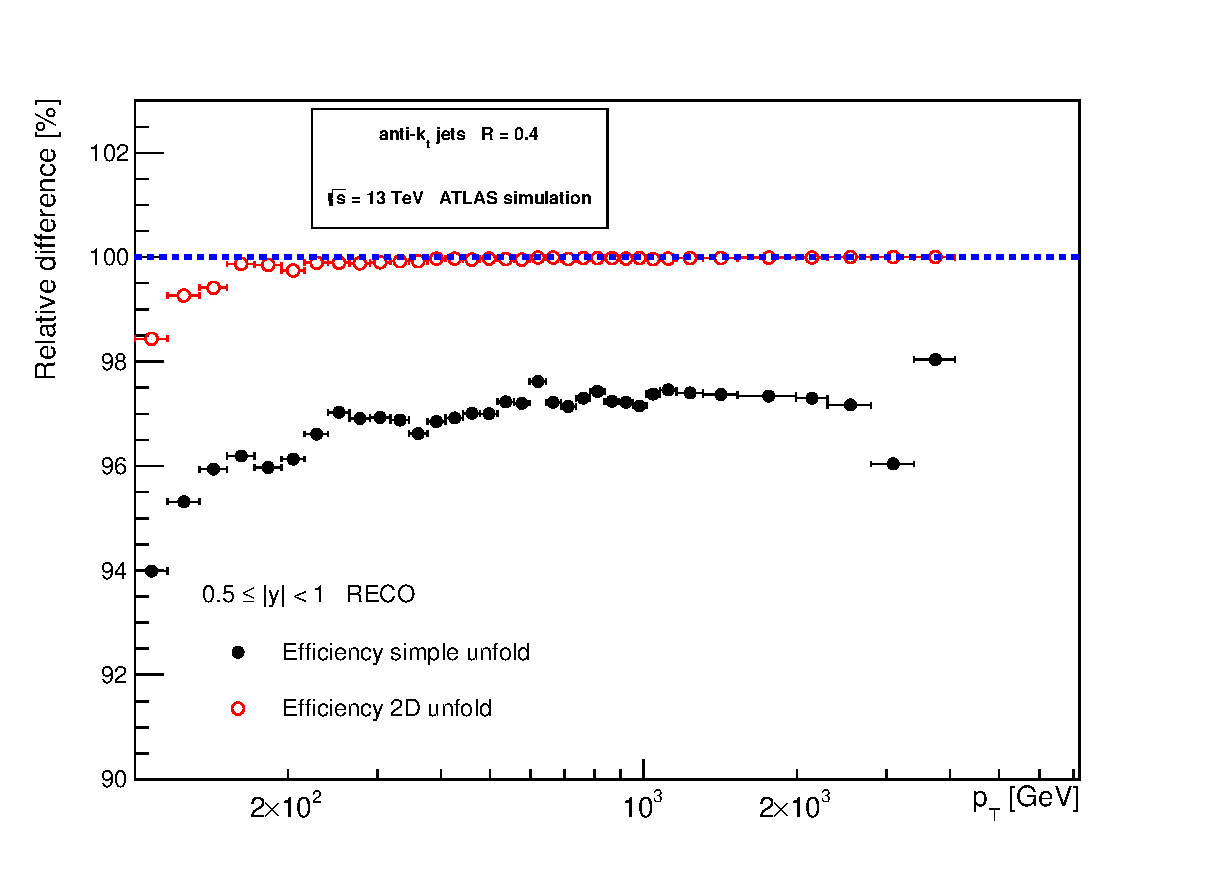
\includegraphics[width=0.49\textwidth]{{Chapter3/MatchEffSimpe2DSignal|abs(y)|0.5-1Compare}.eps}
  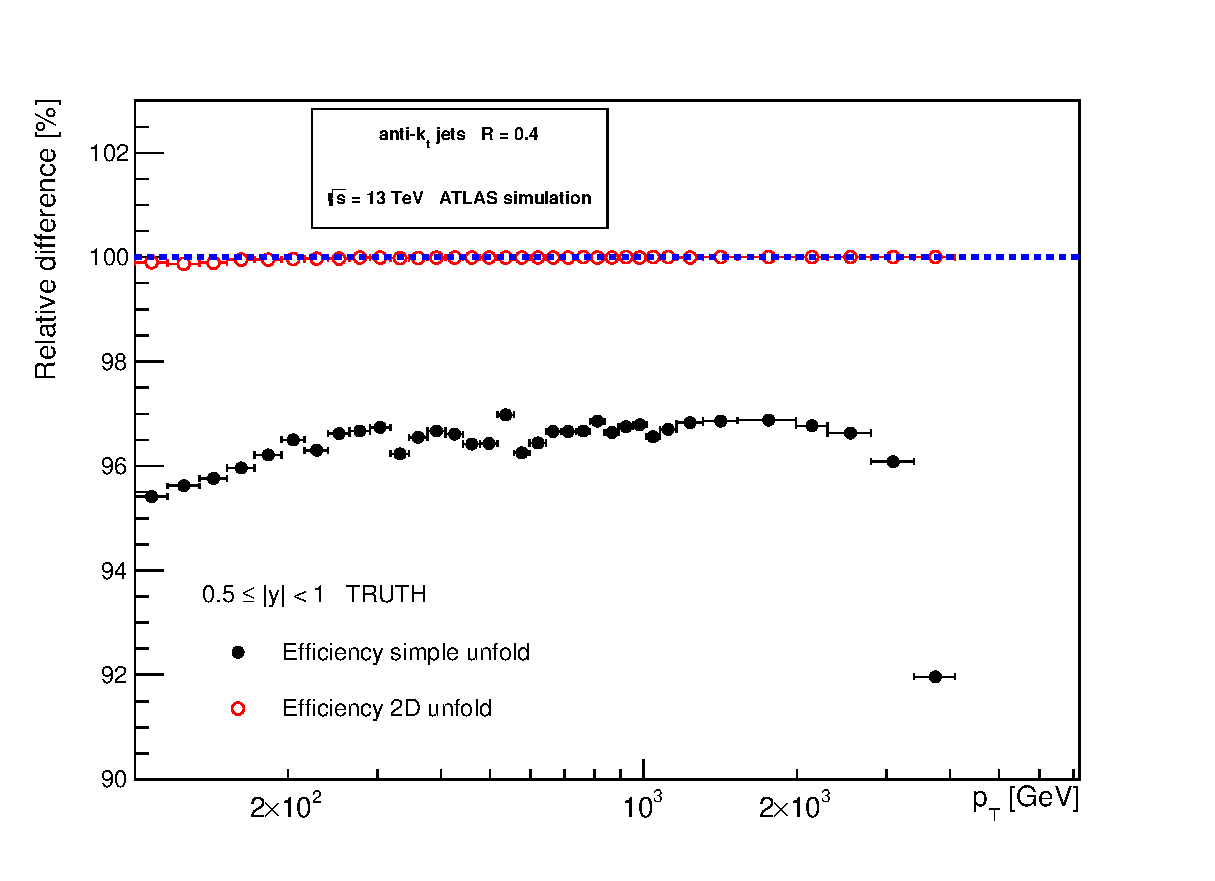
\includegraphics[width=0.49\textwidth]{{Chapter3/MatchEffSimpe2DTruth|abs(y)|0.5-1Compare}.eps}
\end{figure}
\end{center}

\begin{figure}[p]
  \centering
  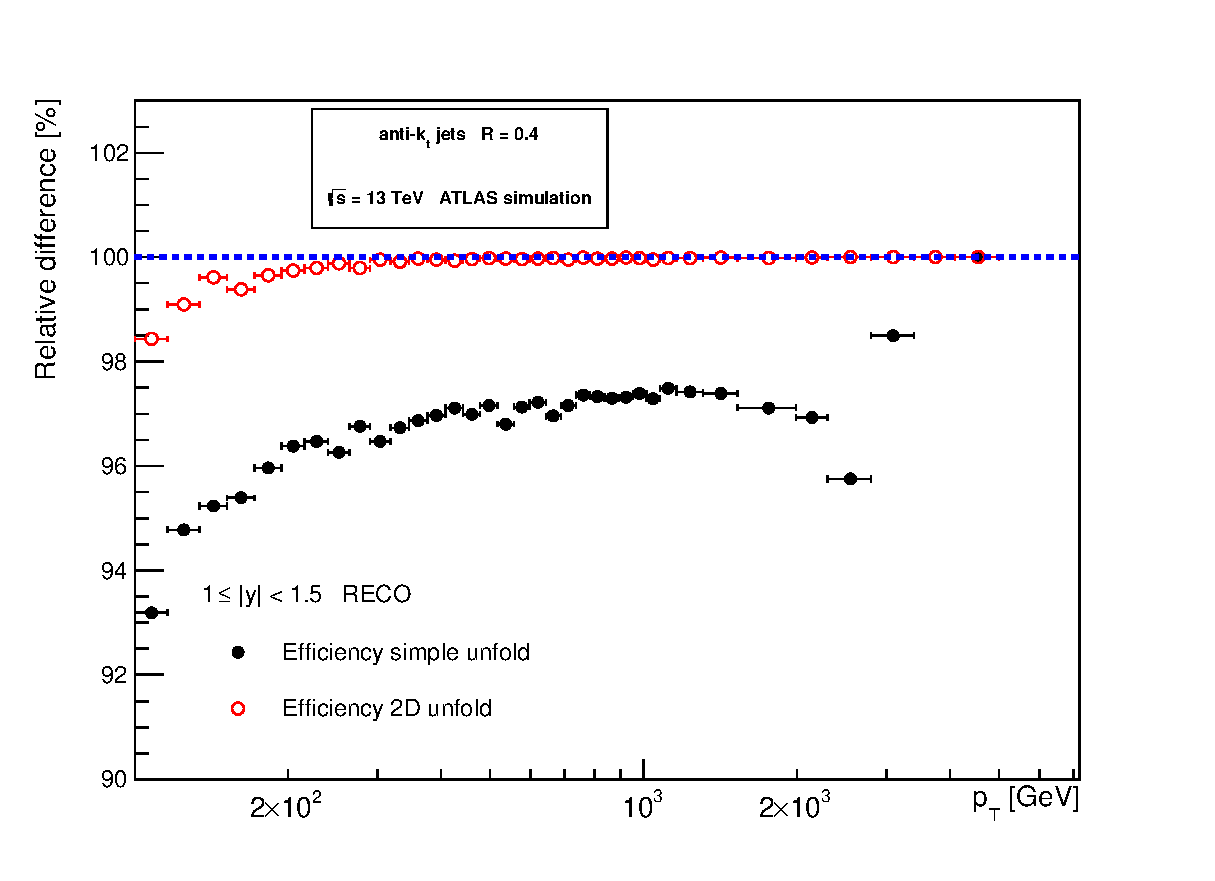
\includegraphics[width=0.49\textwidth]{{Chapter3/MatchEffSimpe2DSignal|abs(y)|1-1.5Compare}.eps}
  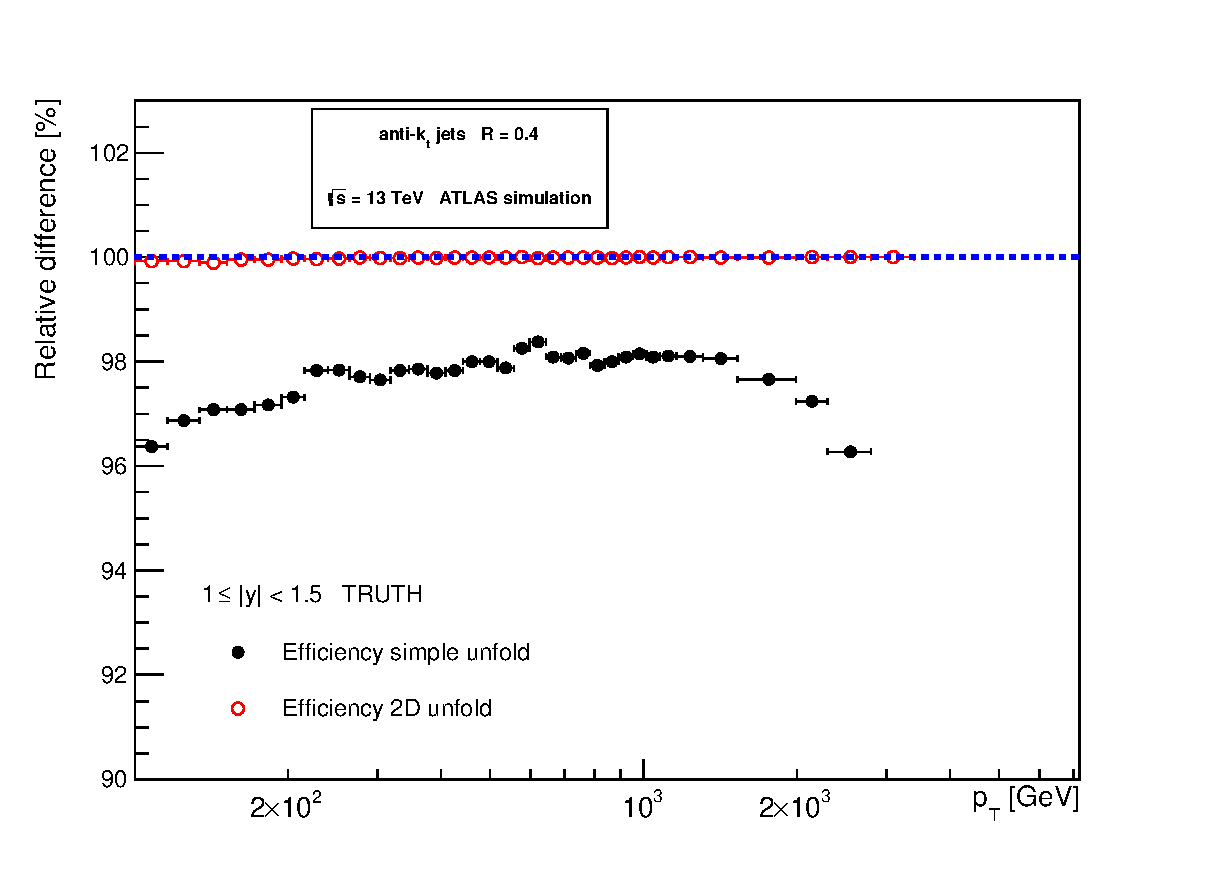
\includegraphics[width=0.49\textwidth]{{Chapter3/MatchEffSimpe2DTruth|abs(y)|1-1.5Compare}.eps}
  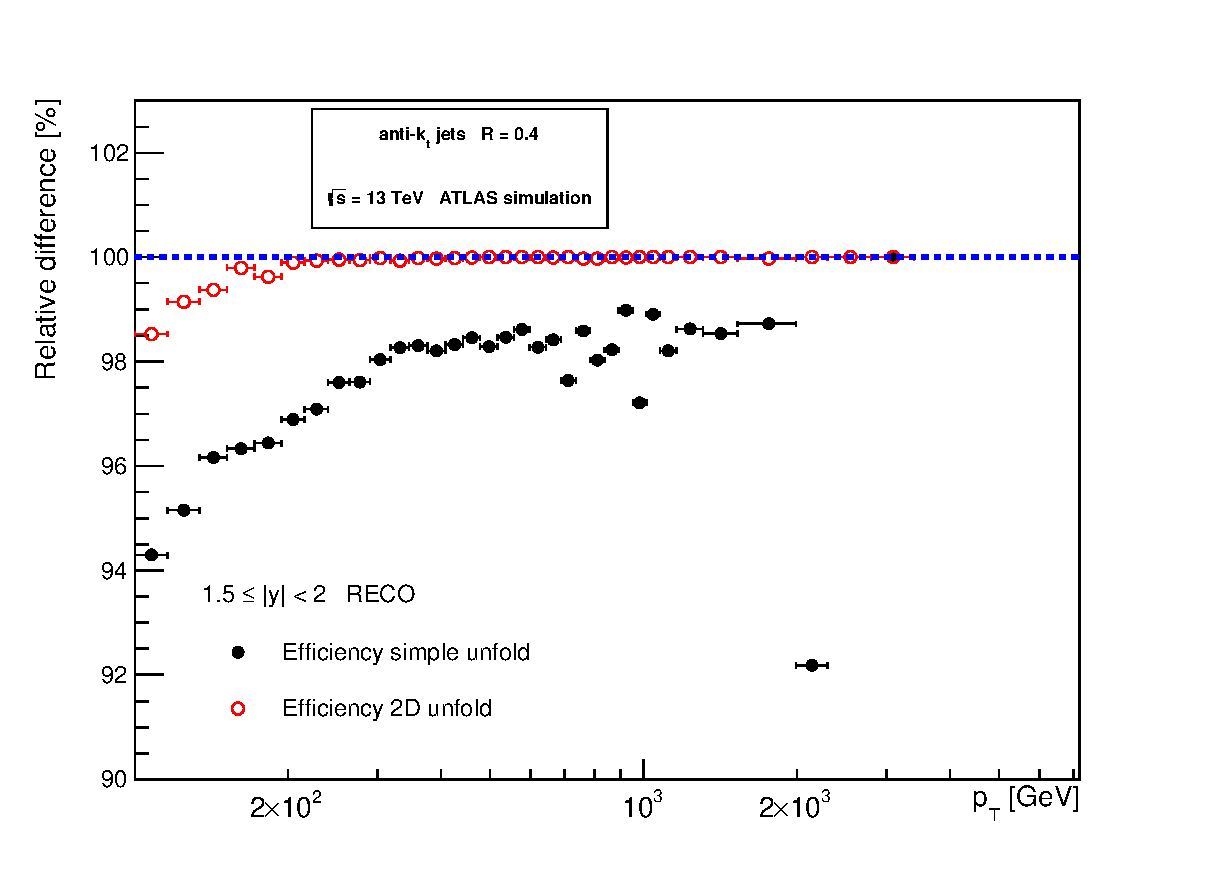
\includegraphics[width=0.49\textwidth]{{Chapter3/MatchEffSimpe2DSignal|abs(y)|1.5-2Compare}.eps}
  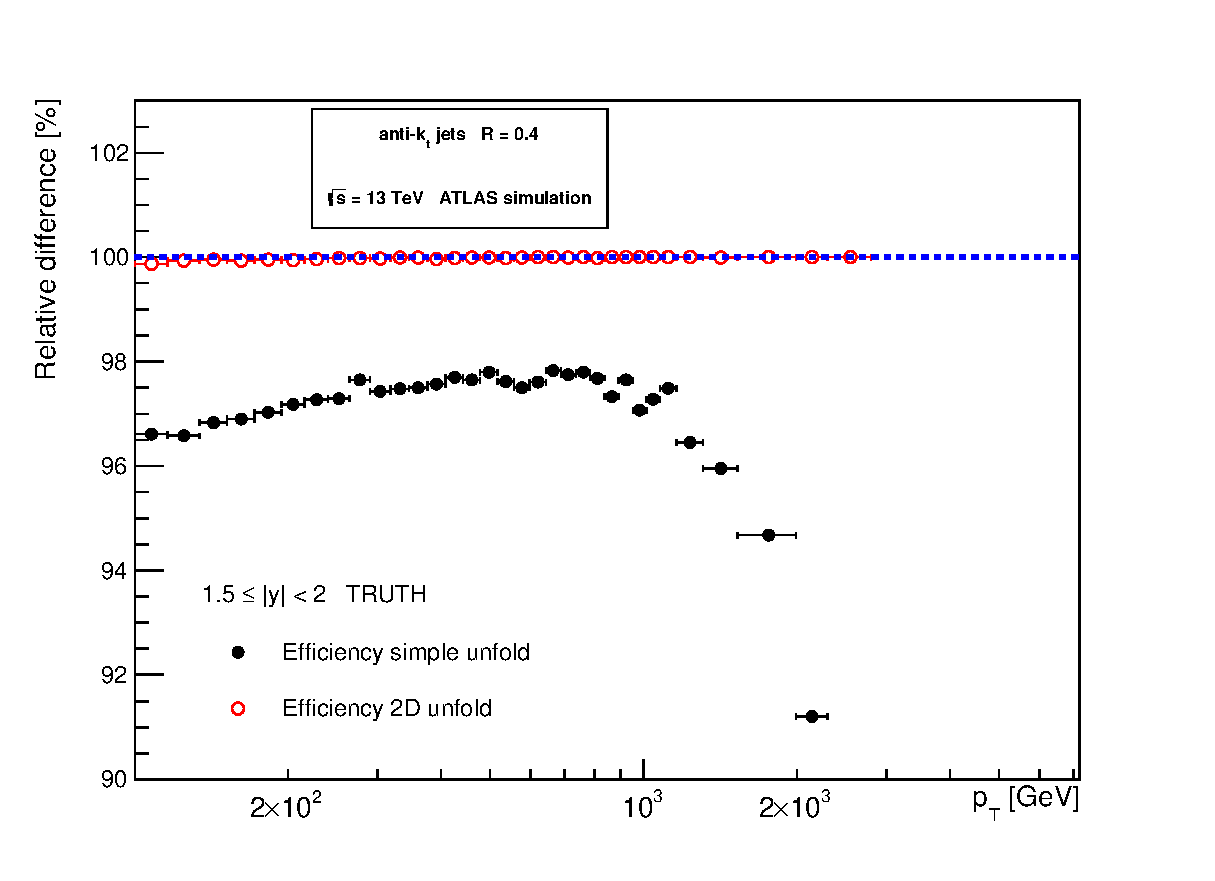
\includegraphics[width=0.49\textwidth]{{Chapter3/MatchEffSimpe2DTruth|abs(y)|1.5-2Compare}.eps}
  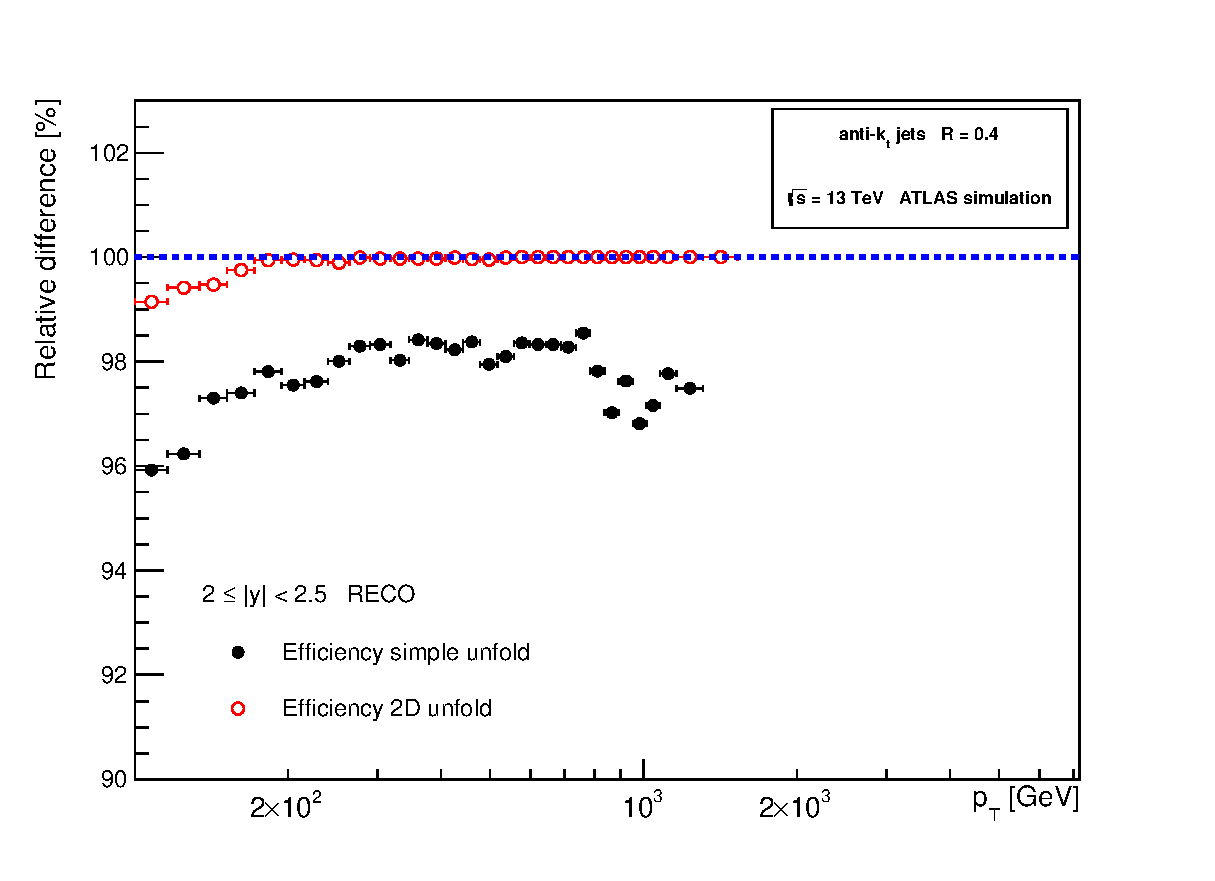
\includegraphics[width=0.49\textwidth]{{Chapter3/MatchEffSimpe2DSignal|abs(y)|2-2.5Compare}.eps}
  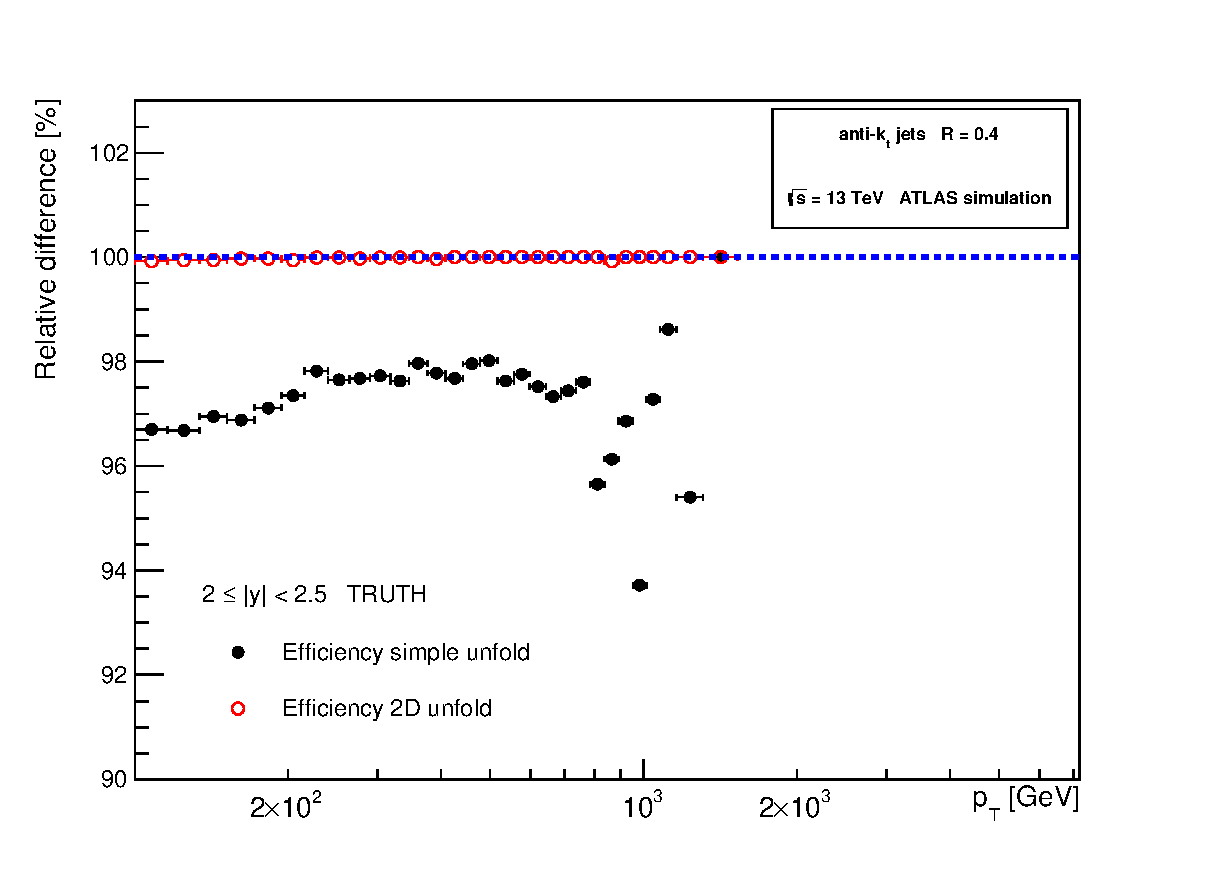
\includegraphics[width=0.49\textwidth]{{Chapter3/MatchEffSimpe2DTruth|abs(y)|2-2.5Compare}.eps}
\end{figure}

\begin{figure}[p]
  \centering
  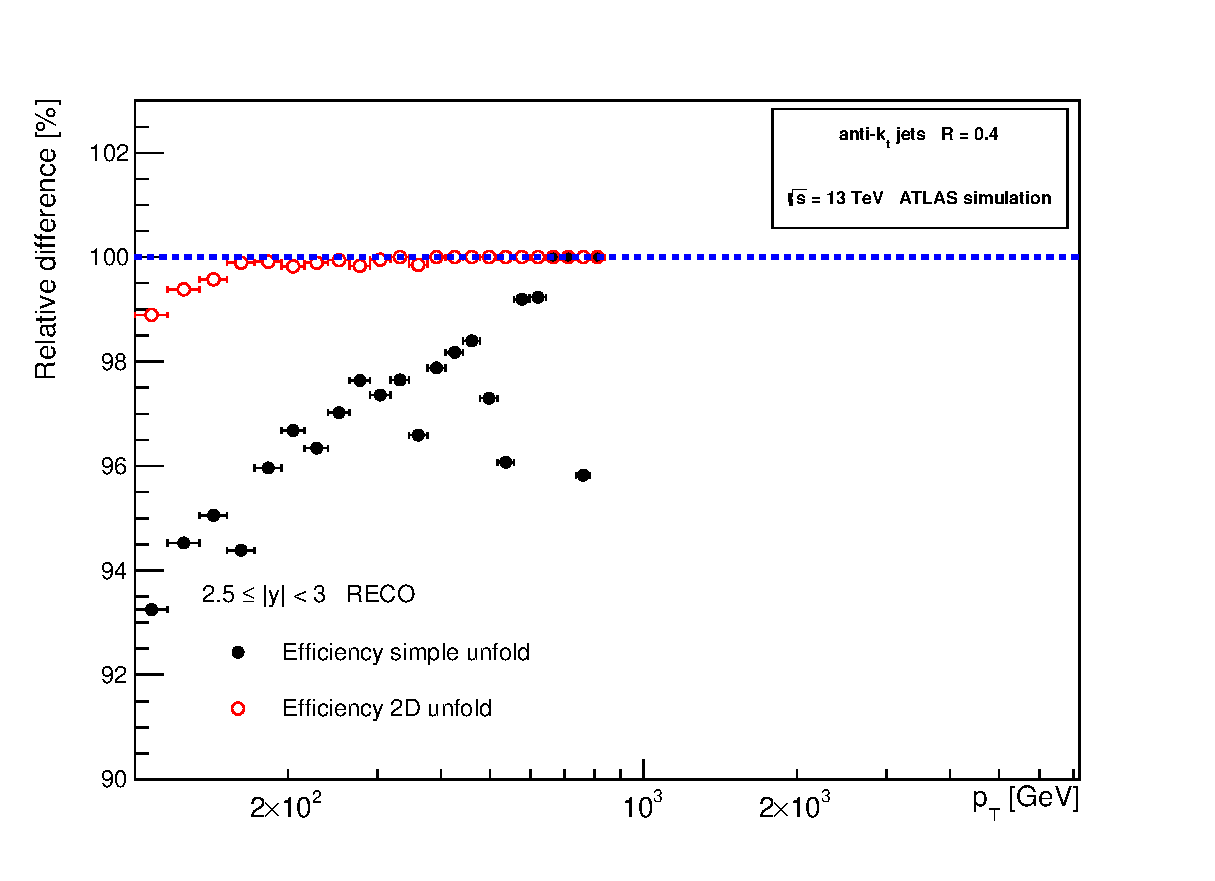
\includegraphics[width=0.49\textwidth]{{Chapter3/MatchEffSimpe2DSignal|abs(y)|2.5-3Compare}.eps}
  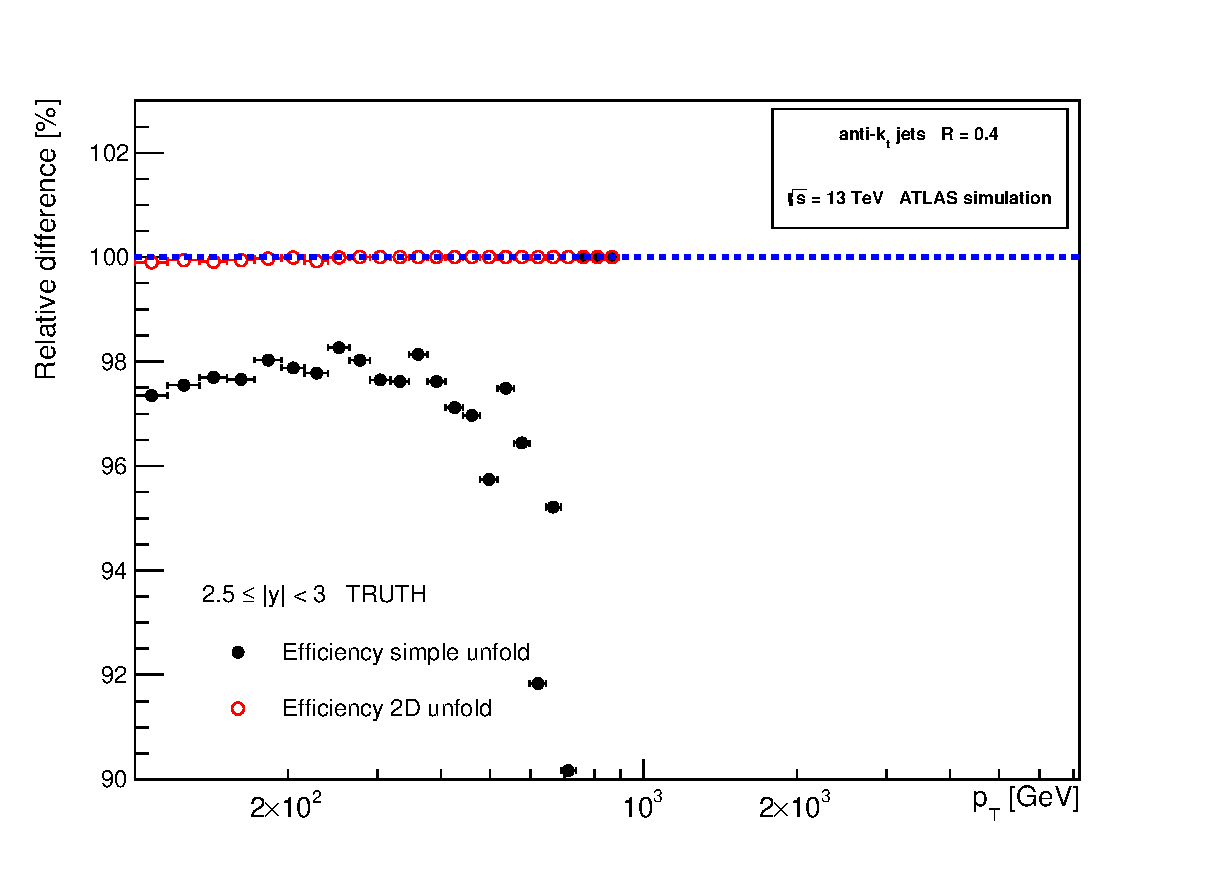
\includegraphics[width=0.49\textwidth]{{Chapter3/MatchEffSimpe2DTruth|abs(y)|2.5-3Compare}.eps}
  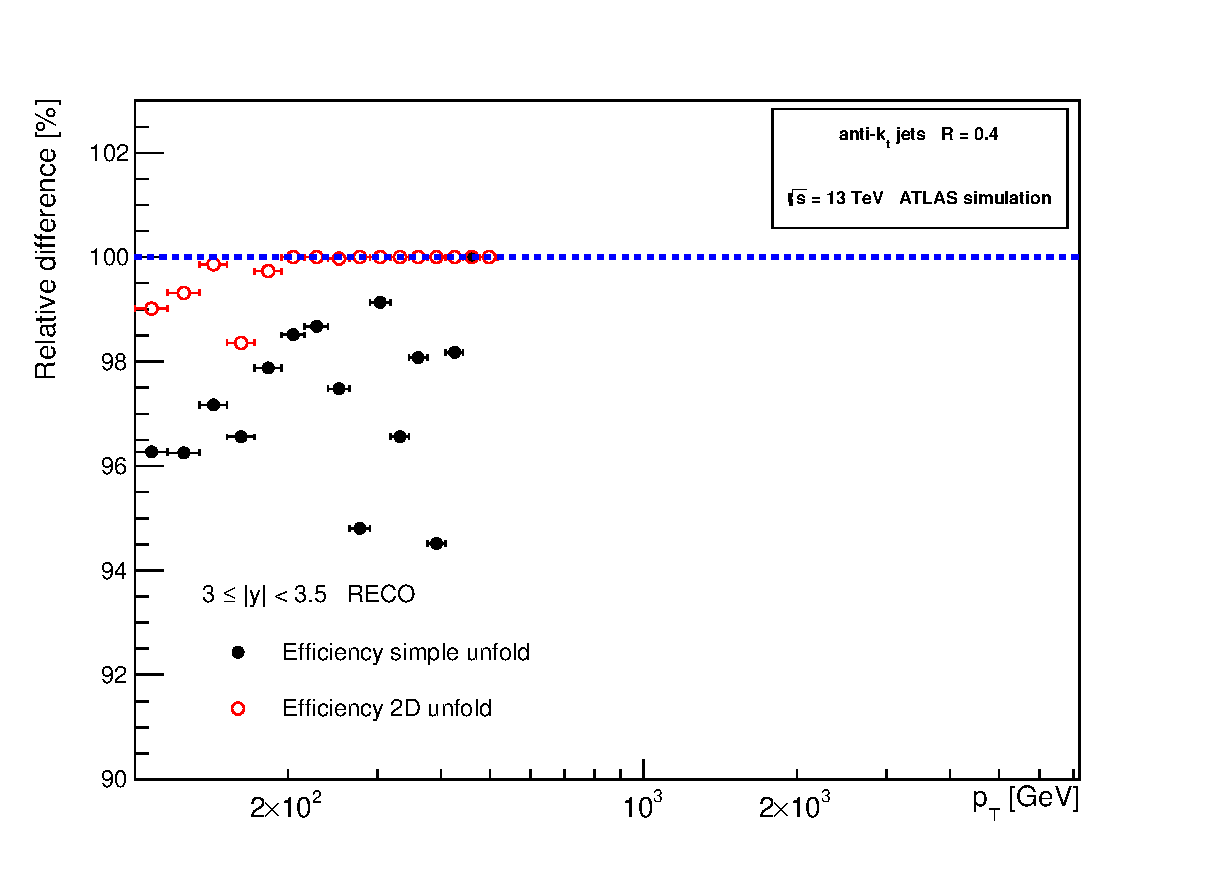
\includegraphics[width=0.49\textwidth]{{Chapter3/MatchEffSimpe2DSignal|abs(y)|3-3.5Compare}.eps}
  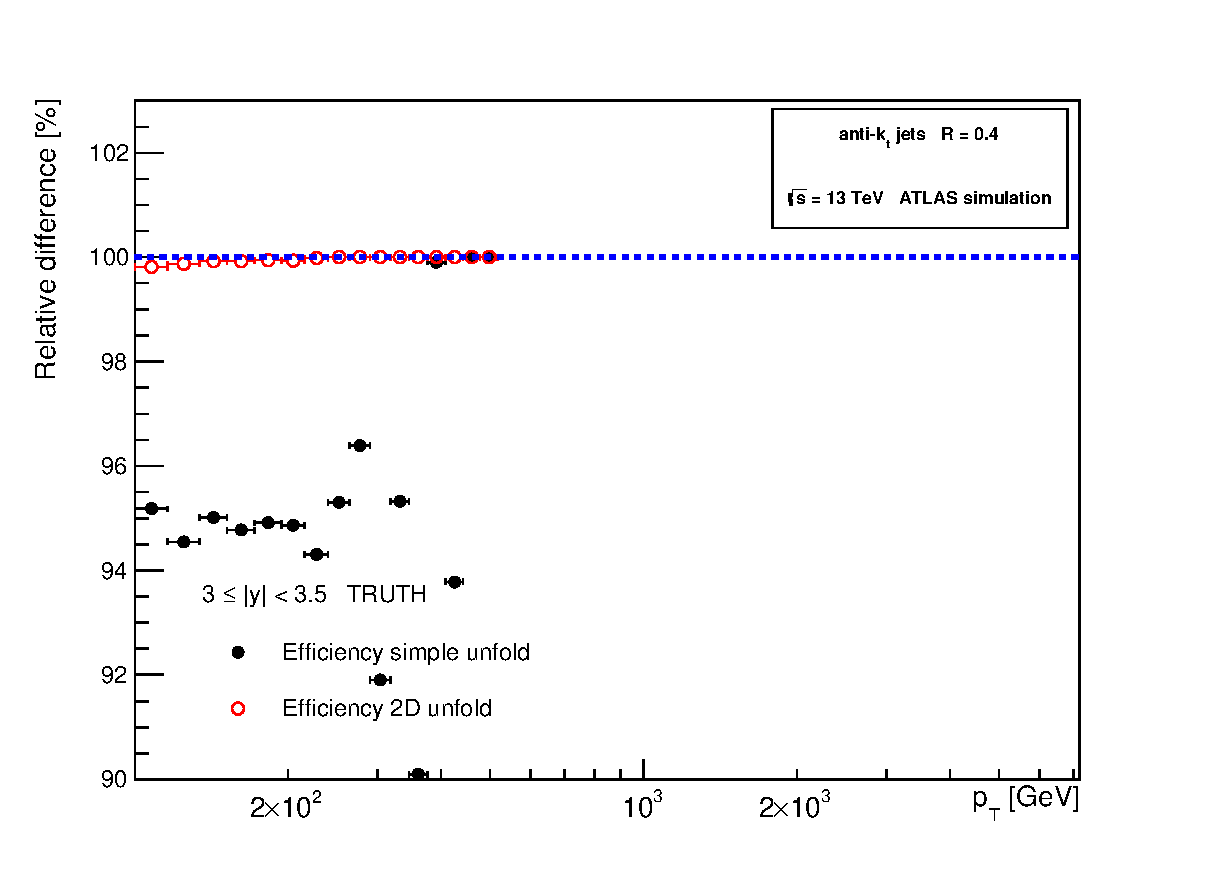
\includegraphics[width=0.49\textwidth]{{Chapter3/MatchEffSimpe2DTruth|abs(y)|3-3.5Compare}.eps}
  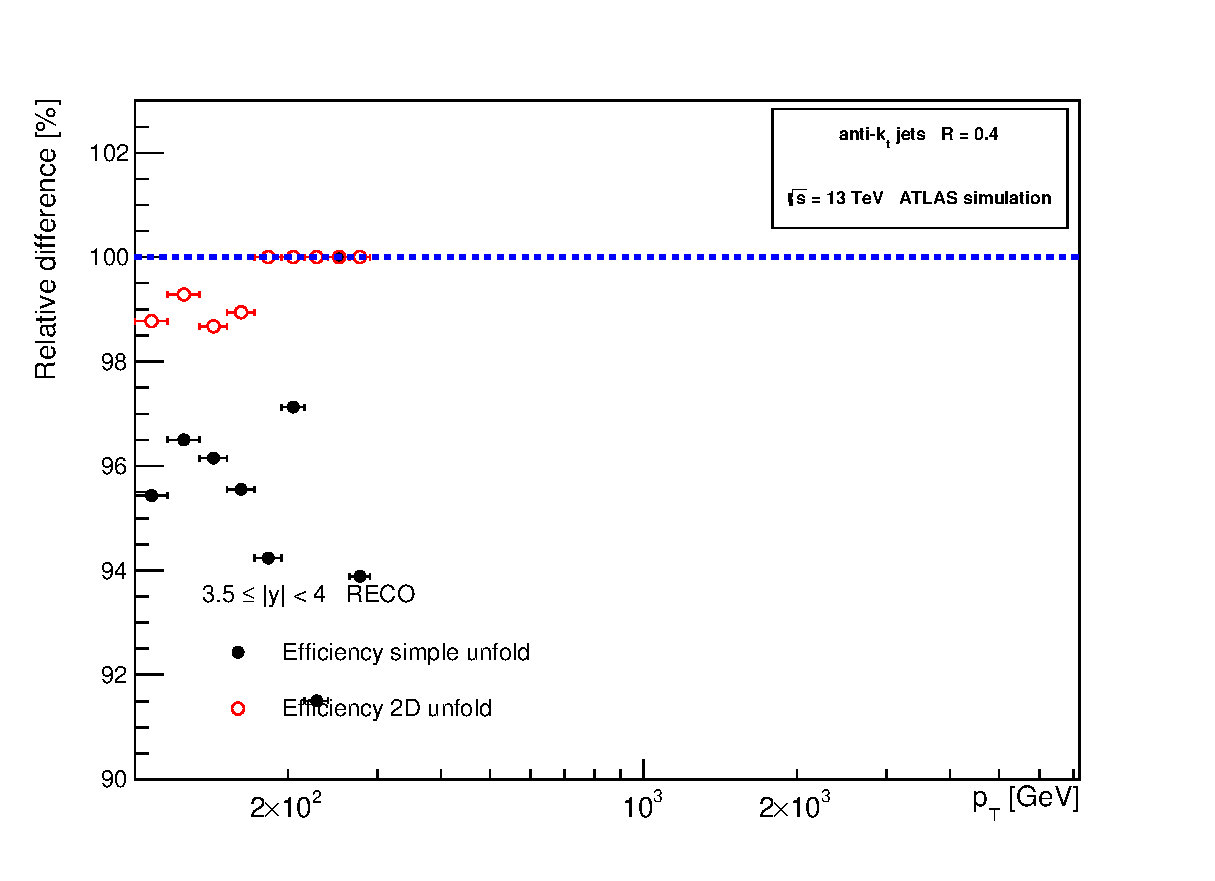
\includegraphics[width=0.49\textwidth]{{Chapter3/MatchEffSimpe2DSignal|abs(y)|3.5-4Compare}.eps}
  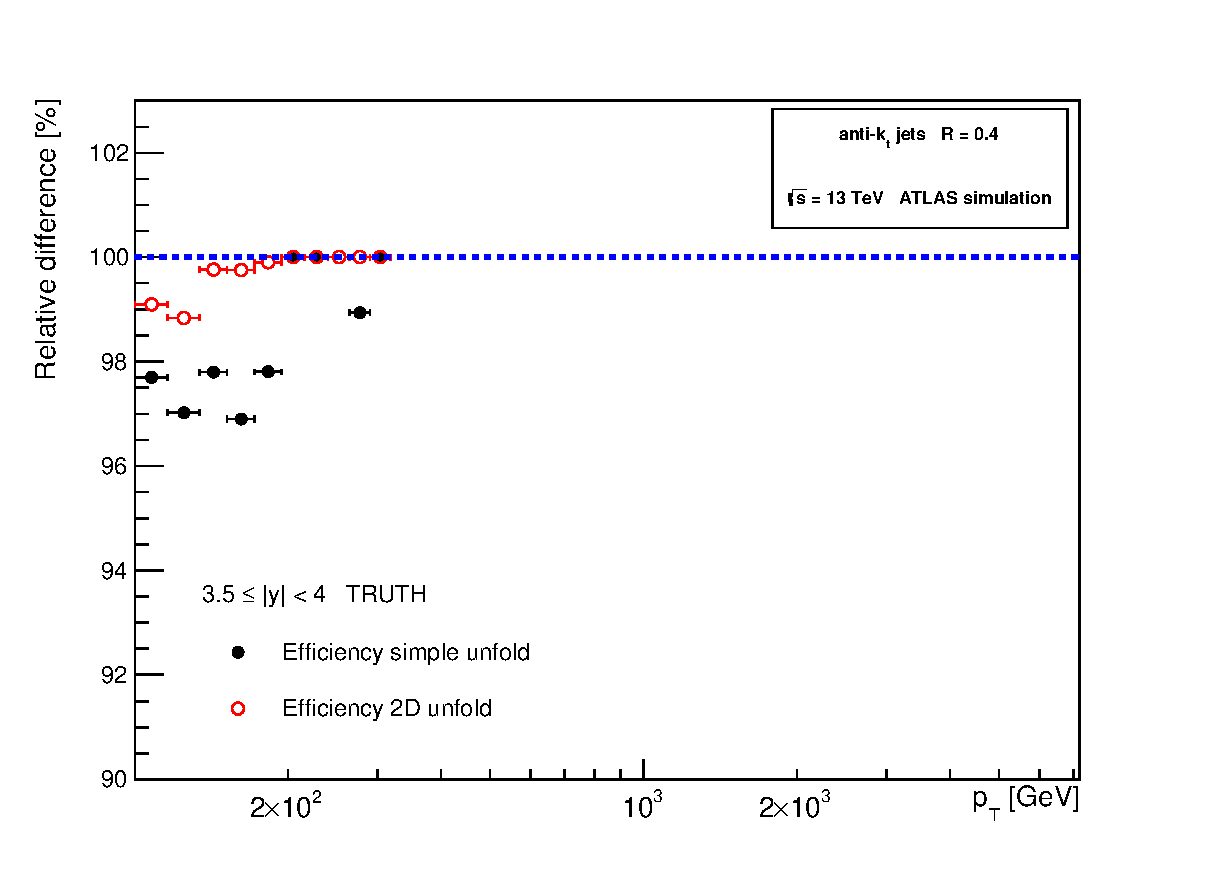
\includegraphics[width=0.49\textwidth]{{Chapter3/MatchEffSimpe2DTruth|abs(y)|3.5-4Compare}.eps}
\end{figure}

\section{Unfolding Results}

\begin{center}
\begin{figure}[H]
  \centering
  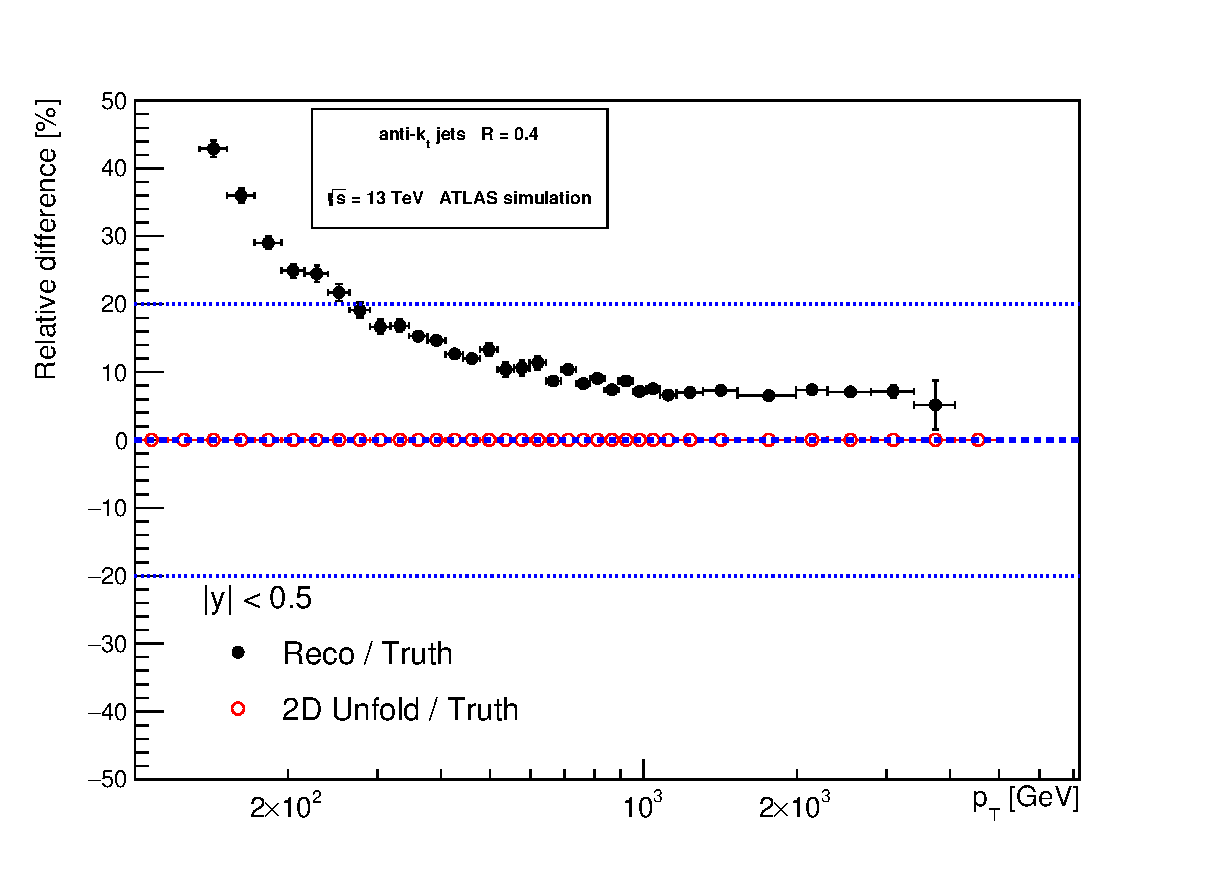
\includegraphics[width=0.49\textwidth]{{Chapter3/SignalUnfolded_VS_Truth|abs(y)|0-0.5Compare}.eps}
  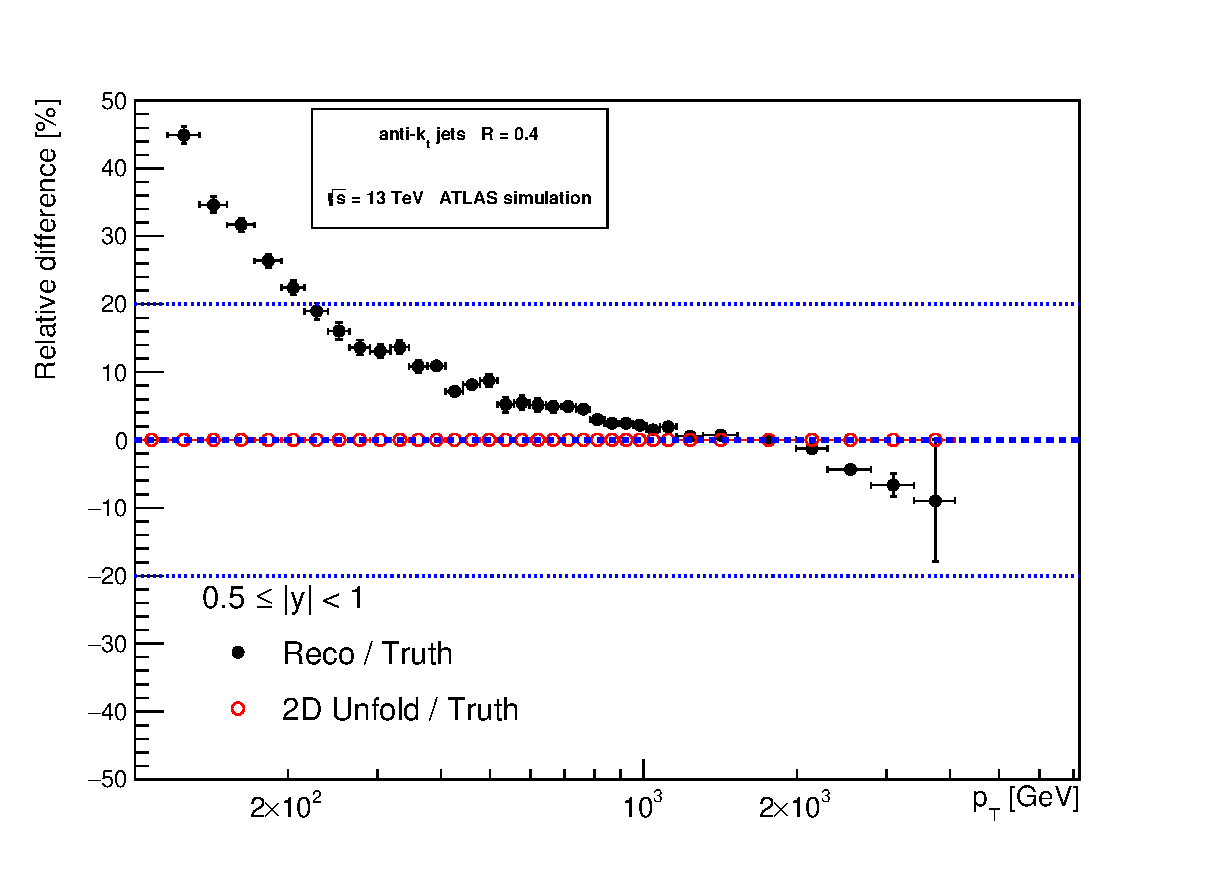
\includegraphics[width=0.49\textwidth]{{Chapter3/SignalUnfolded_VS_Truth|abs(y)|0.5-1Compare}.eps}
  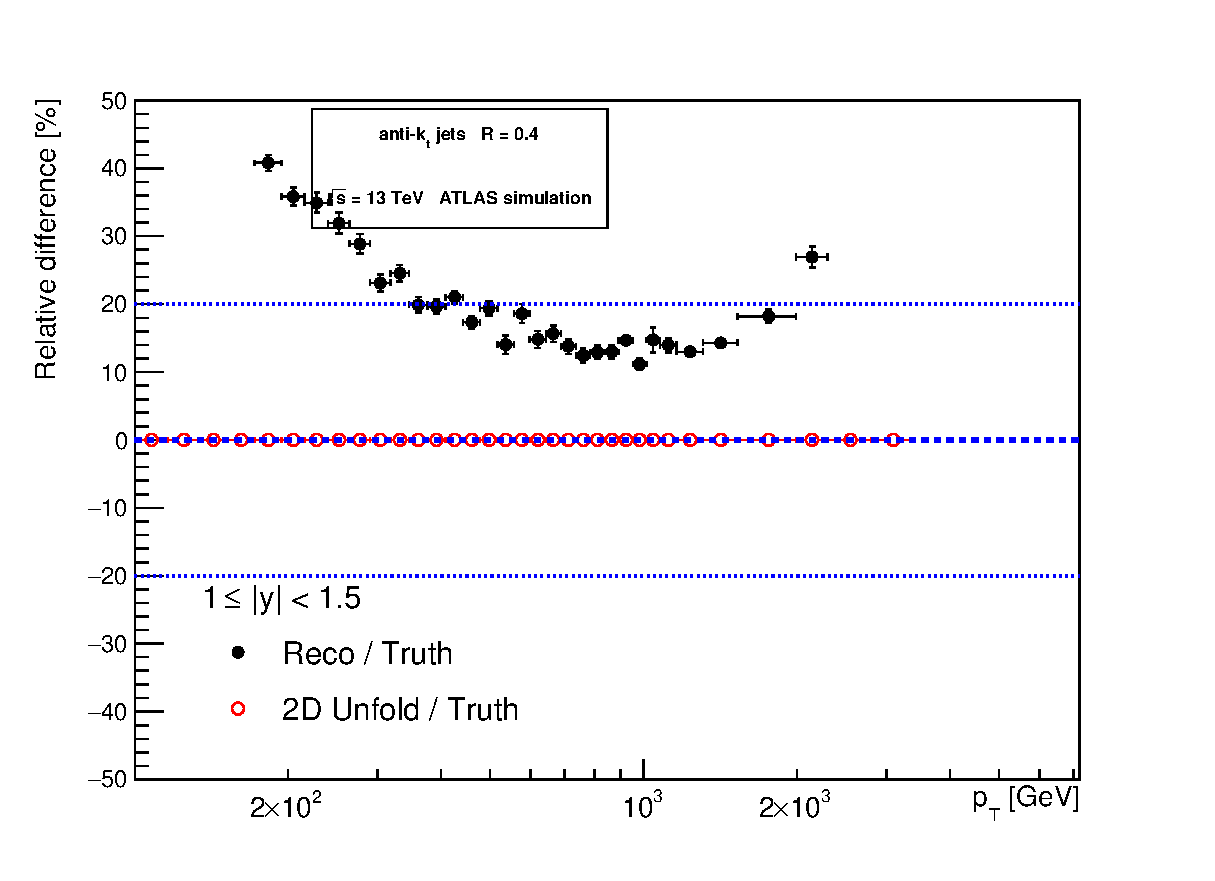
\includegraphics[width=0.49\textwidth]{{Chapter3/SignalUnfolded_VS_Truth|abs(y)|1-1.5Compare}.eps}
  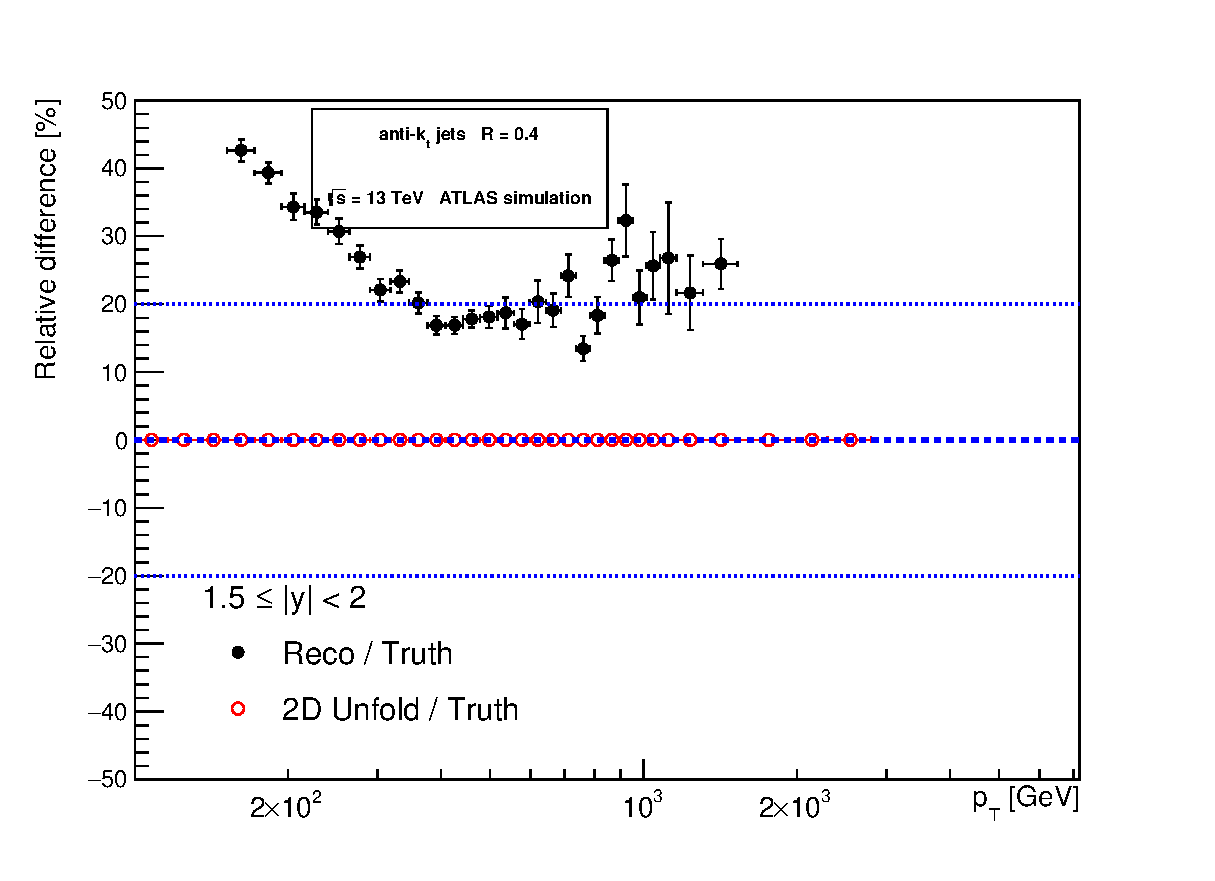
\includegraphics[width=0.49\textwidth]{{Chapter3/SignalUnfolded_VS_Truth|abs(y)|1.5-2Compare}.eps}
\end{figure}
\end{center}

\begin{figure}[p]
  \centering
  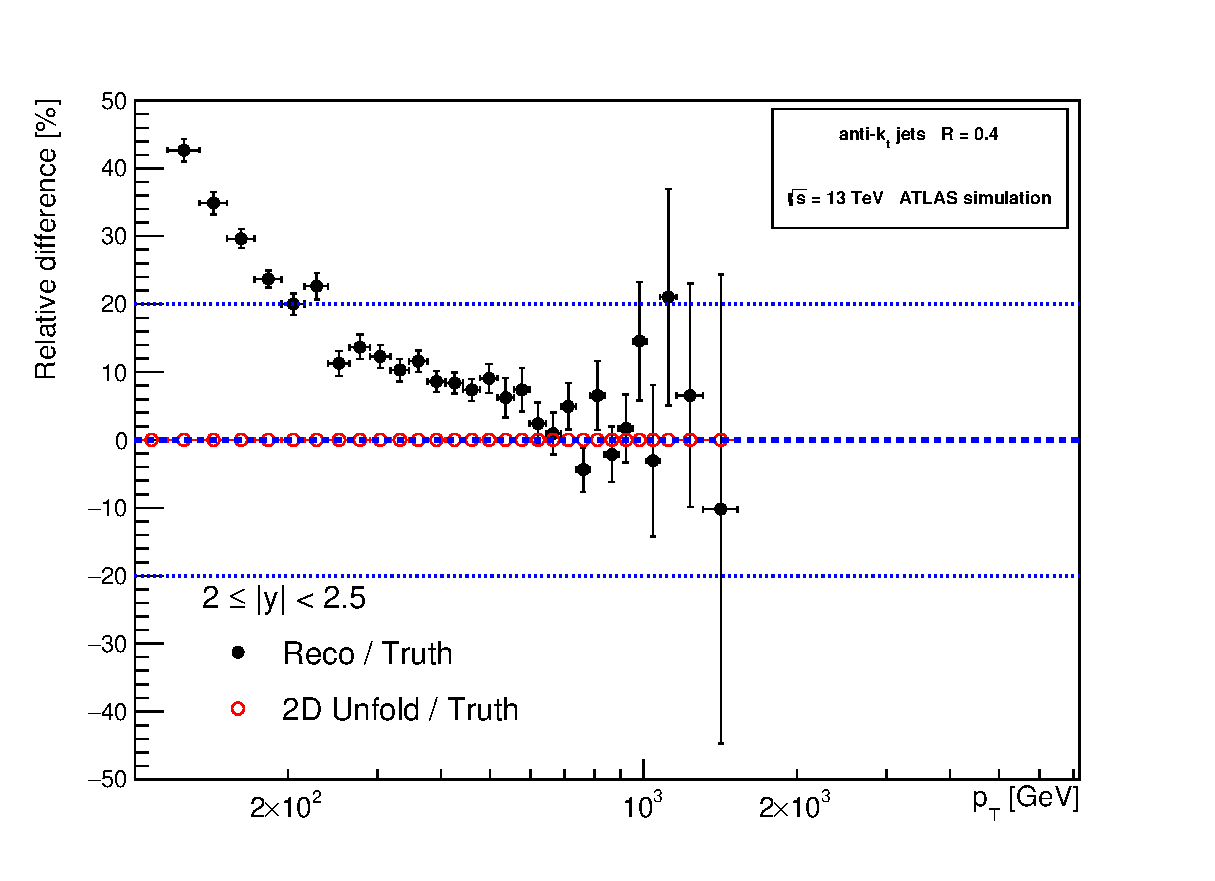
\includegraphics[width=0.49\textwidth]{{Chapter3/SignalUnfolded_VS_Truth|abs(y)|2-2.5Compare}.eps}
  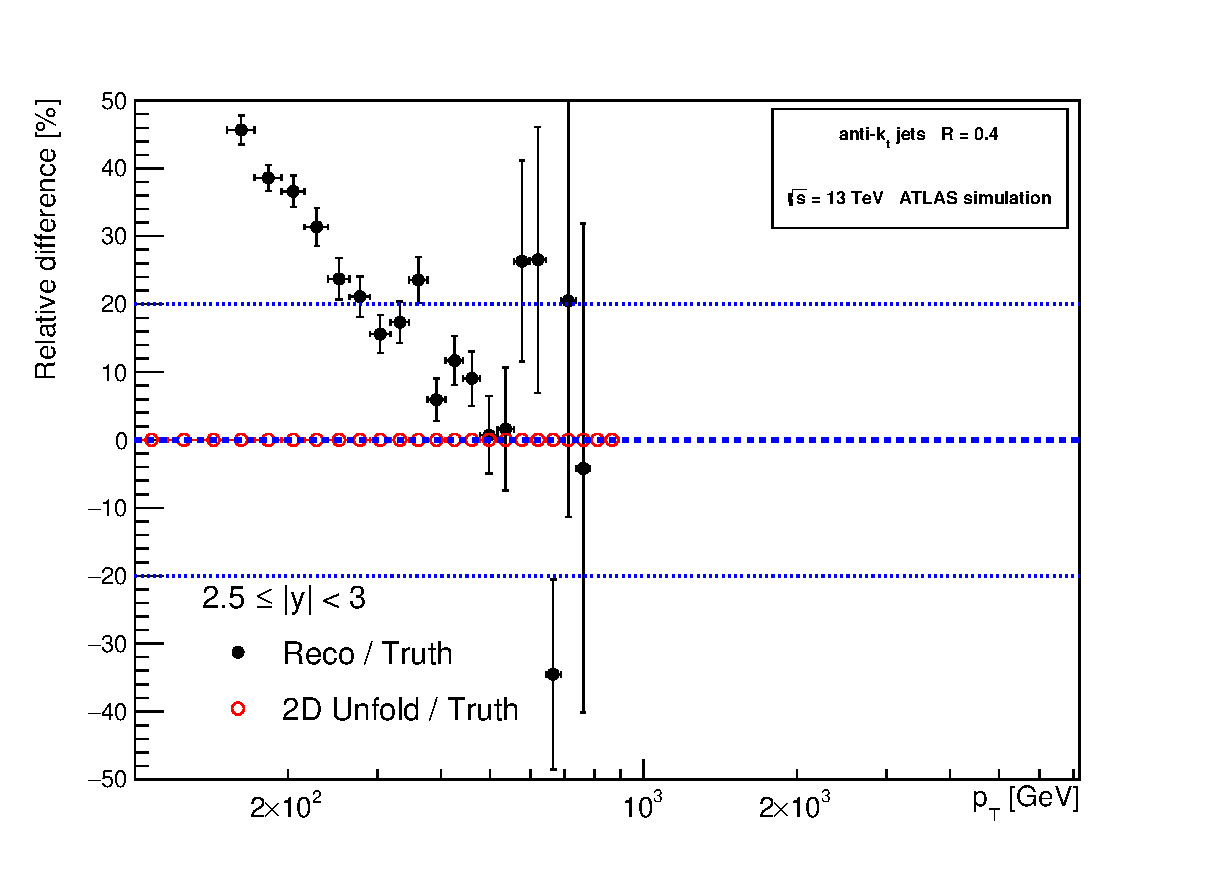
\includegraphics[width=0.49\textwidth]{{Chapter3/SignalUnfolded_VS_Truth|abs(y)|2.5-3Compare}.eps}
  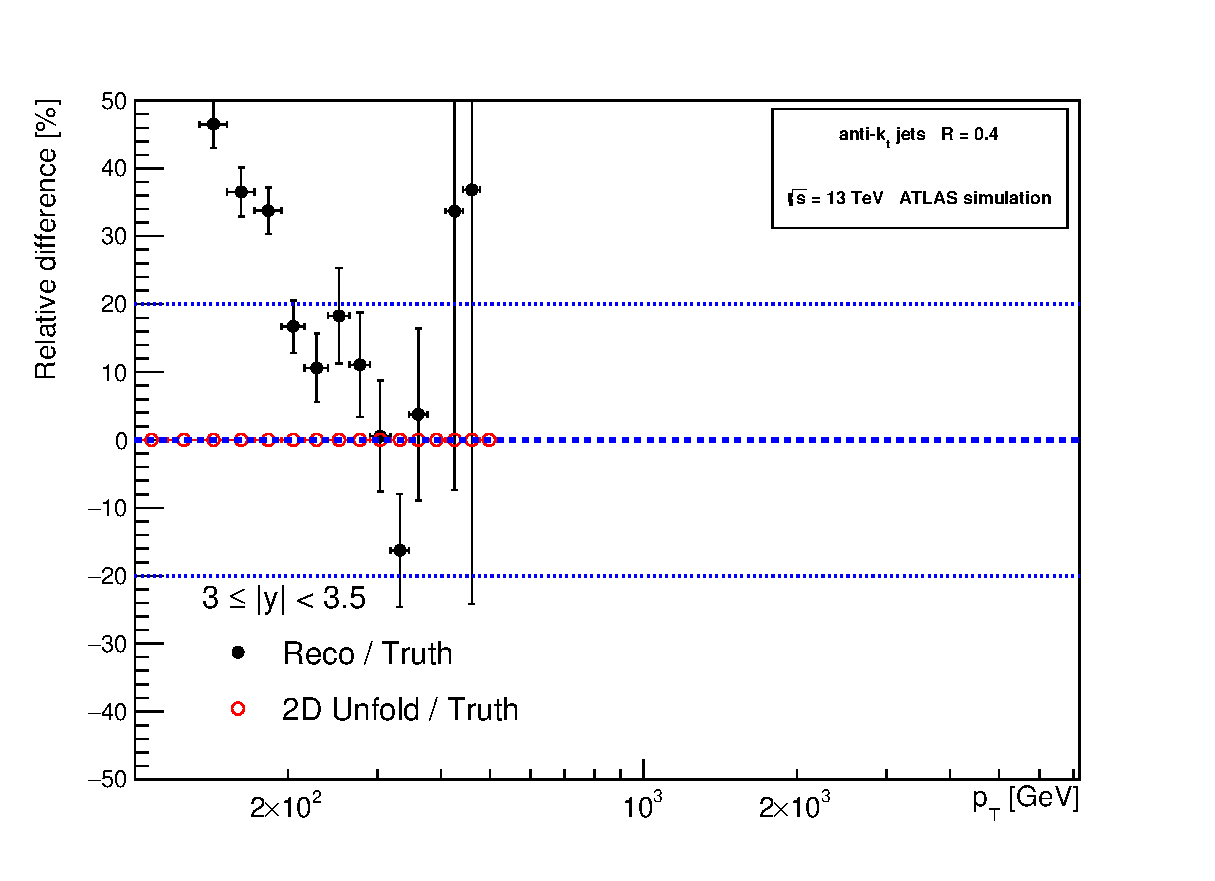
\includegraphics[width=0.49\textwidth]{{Chapter3/SignalUnfolded_VS_Truth|abs(y)|3-3.5Compare}.eps}
  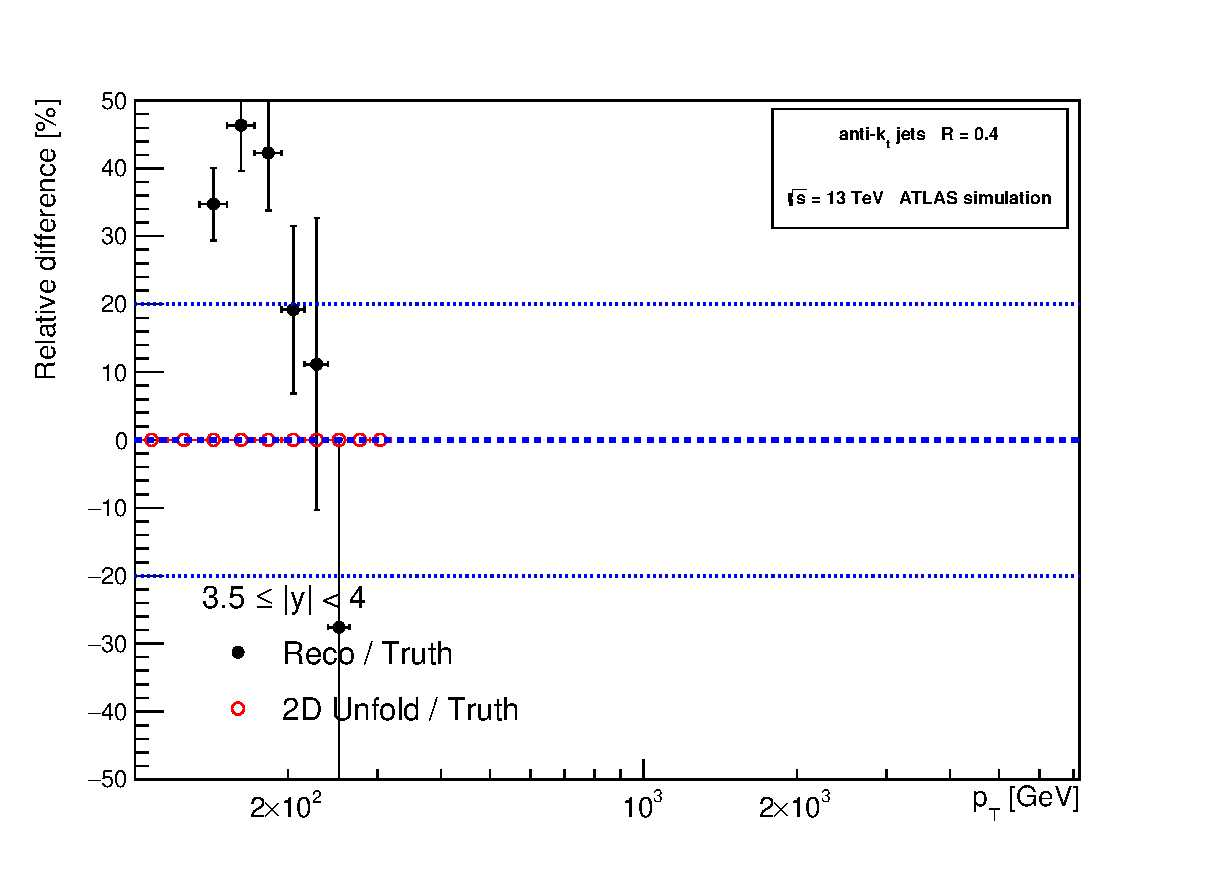
\includegraphics[width=0.49\textwidth]{{Chapter3/SignalUnfolded_VS_Truth|abs(y)|3.5-4Compare}.eps}
\end{figure}

\section{Simple and 2D Unfolding}

\begin{center}
\begin{figure}[H]
  \centering
  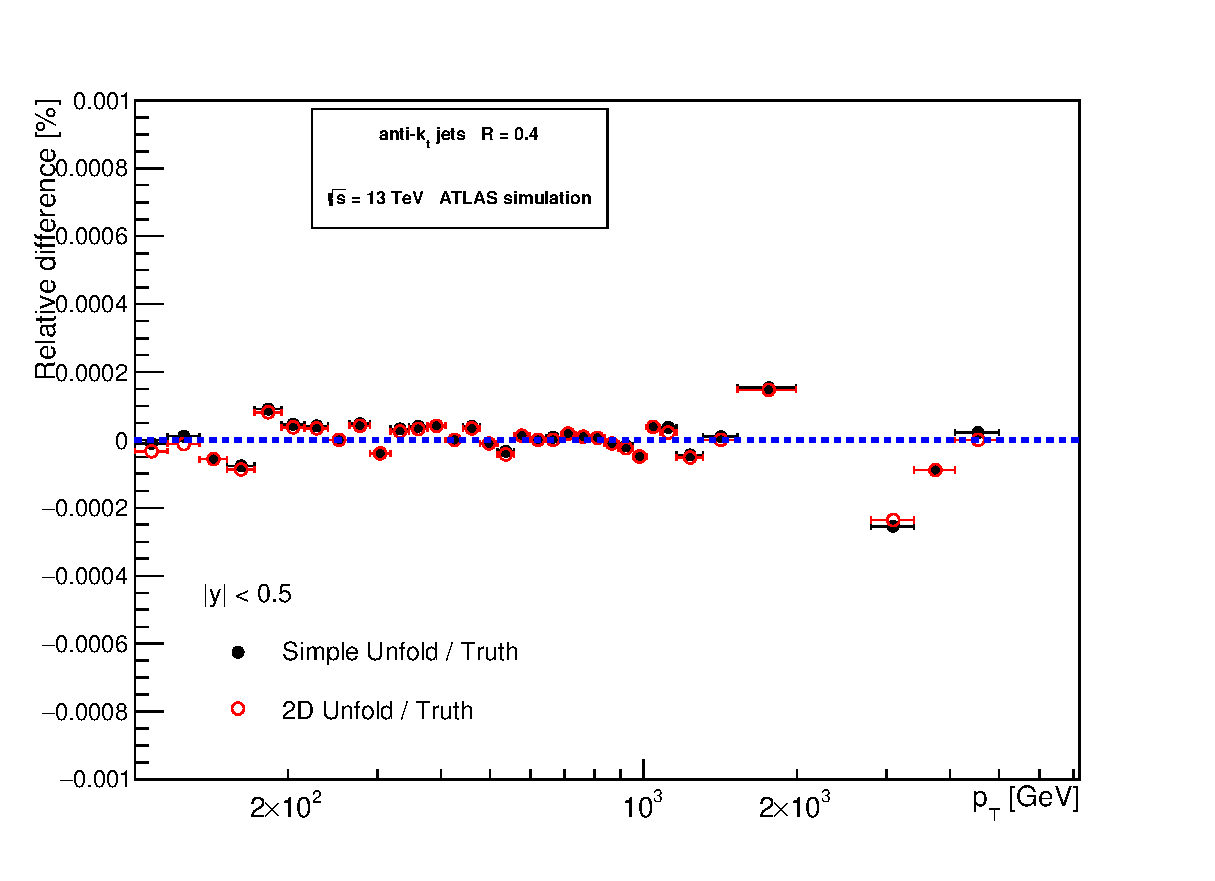
\includegraphics[width=0.49\textwidth]{{Chapter3/UnfoldedSimpleComplex_VS_Truth|abs(y)|0-0.5Compare}.eps}
  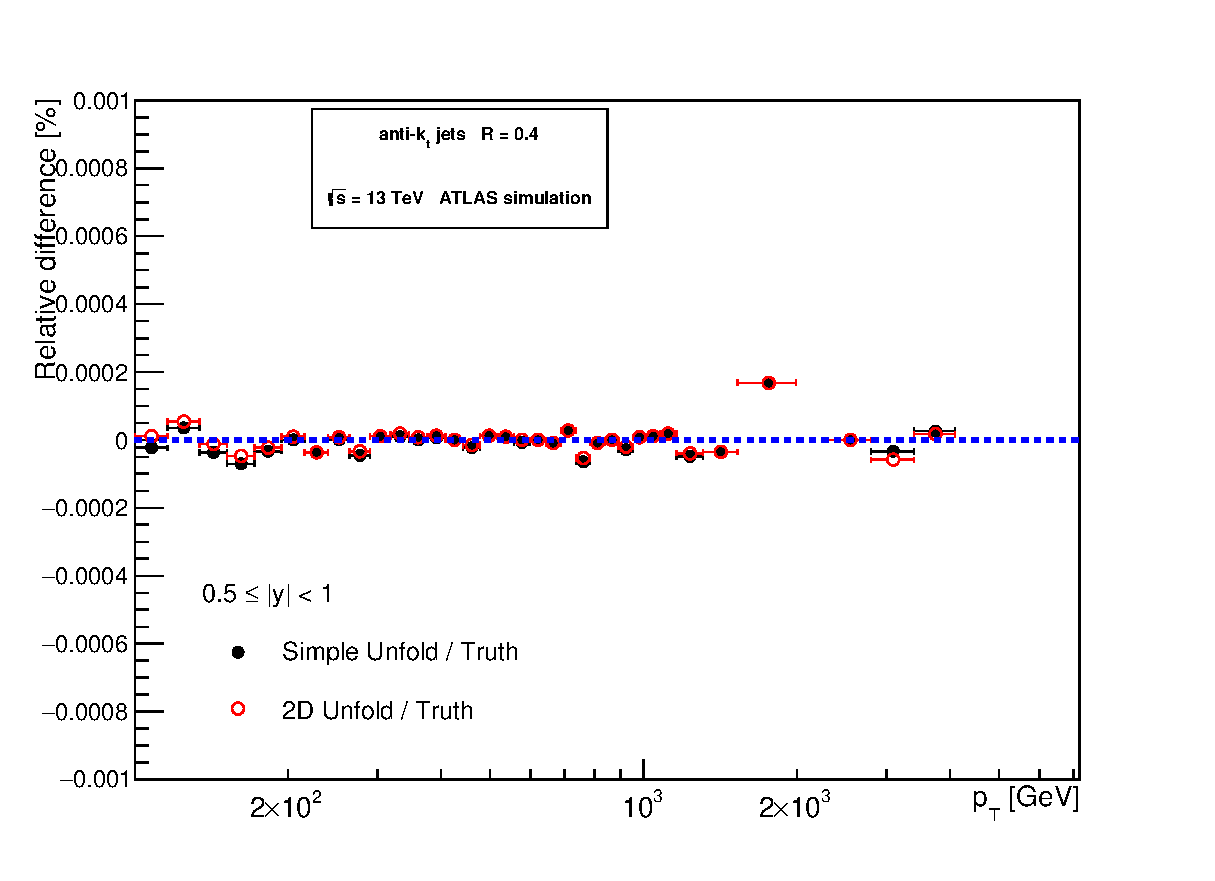
\includegraphics[width=0.49\textwidth]{{Chapter3/UnfoldedSimpleComplex_VS_Truth|abs(y)|0.5-1Compare}.eps}
  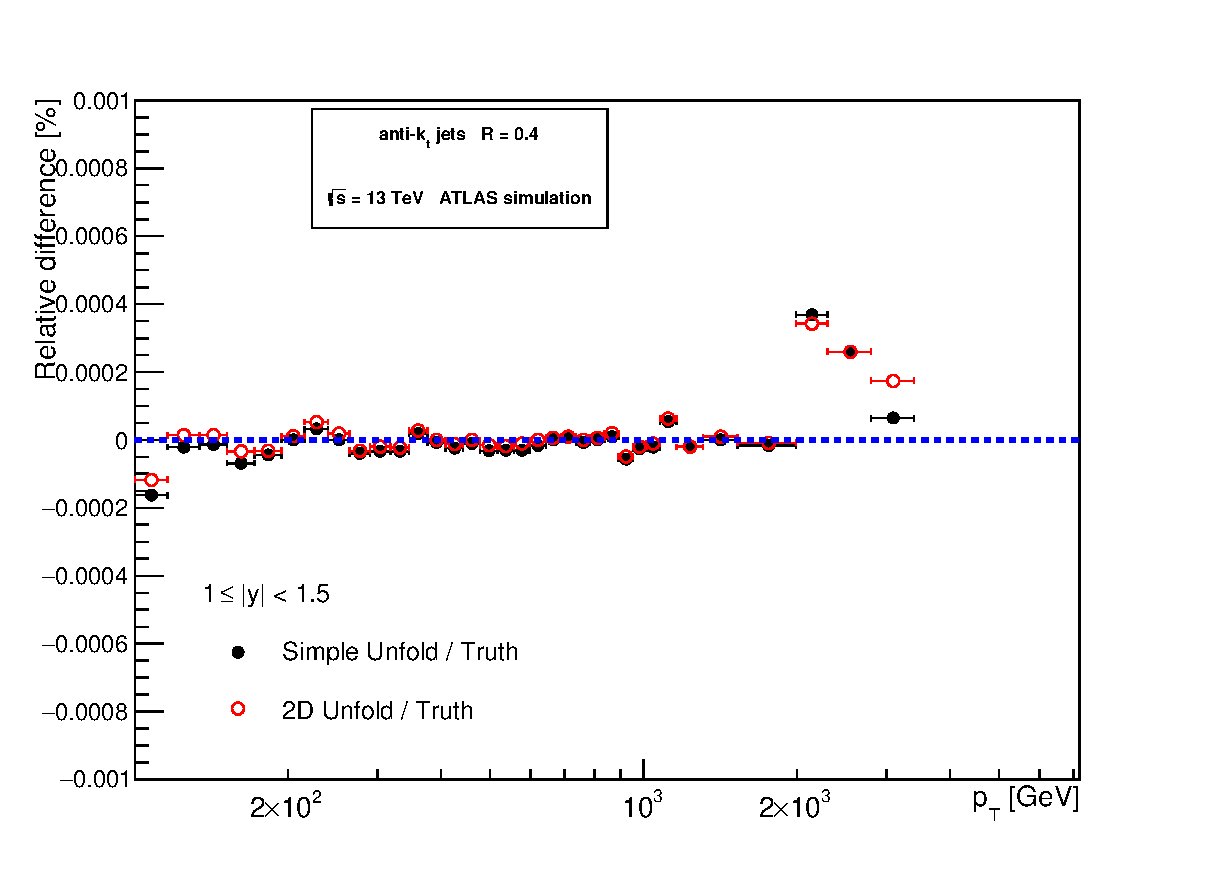
\includegraphics[width=0.49\textwidth]{{Chapter3/UnfoldedSimpleComplex_VS_Truth|abs(y)|1-1.5Compare}.eps}
  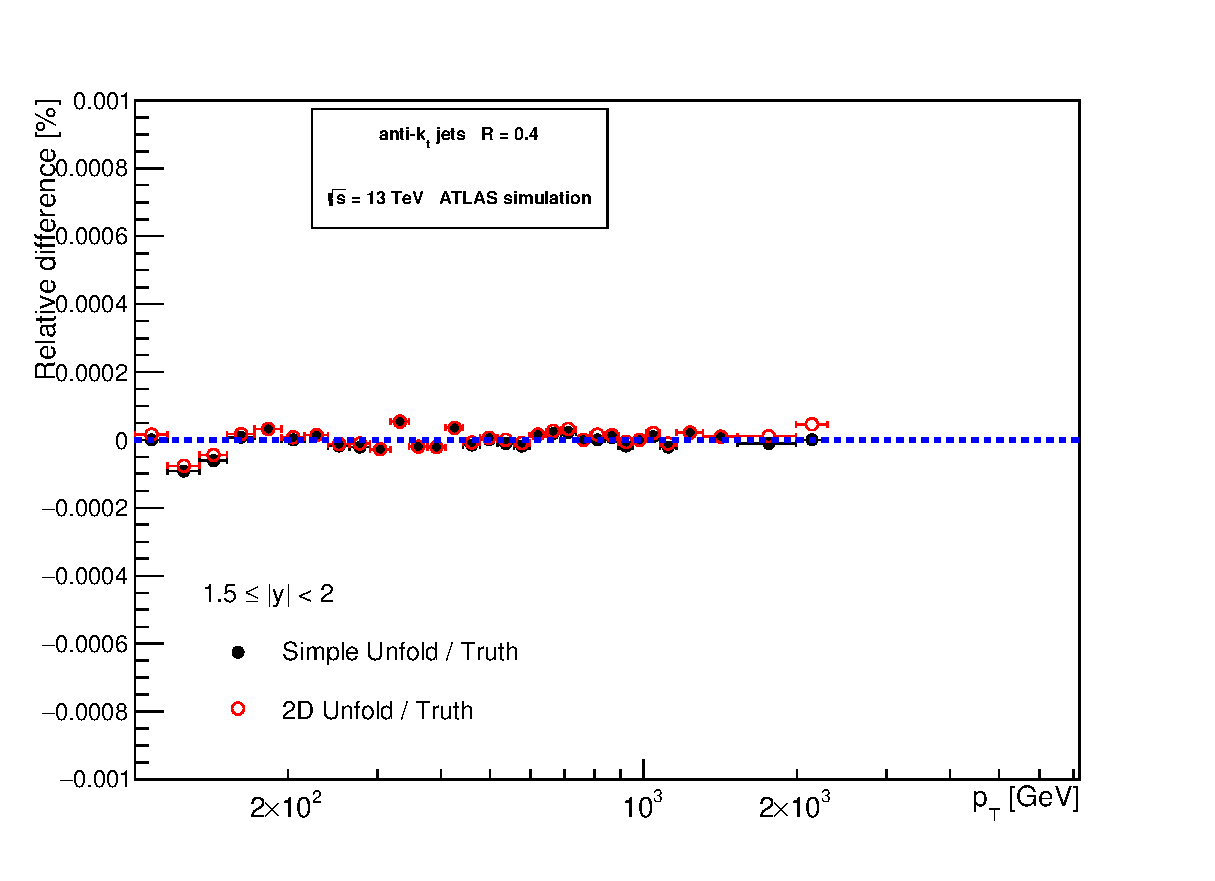
\includegraphics[width=0.49\textwidth]{{Chapter3/UnfoldedSimpleComplex_VS_Truth|abs(y)|1.5-2Compare}.eps}
\end{figure}
\end{center}

\begin{figure}[p]
  \centering
  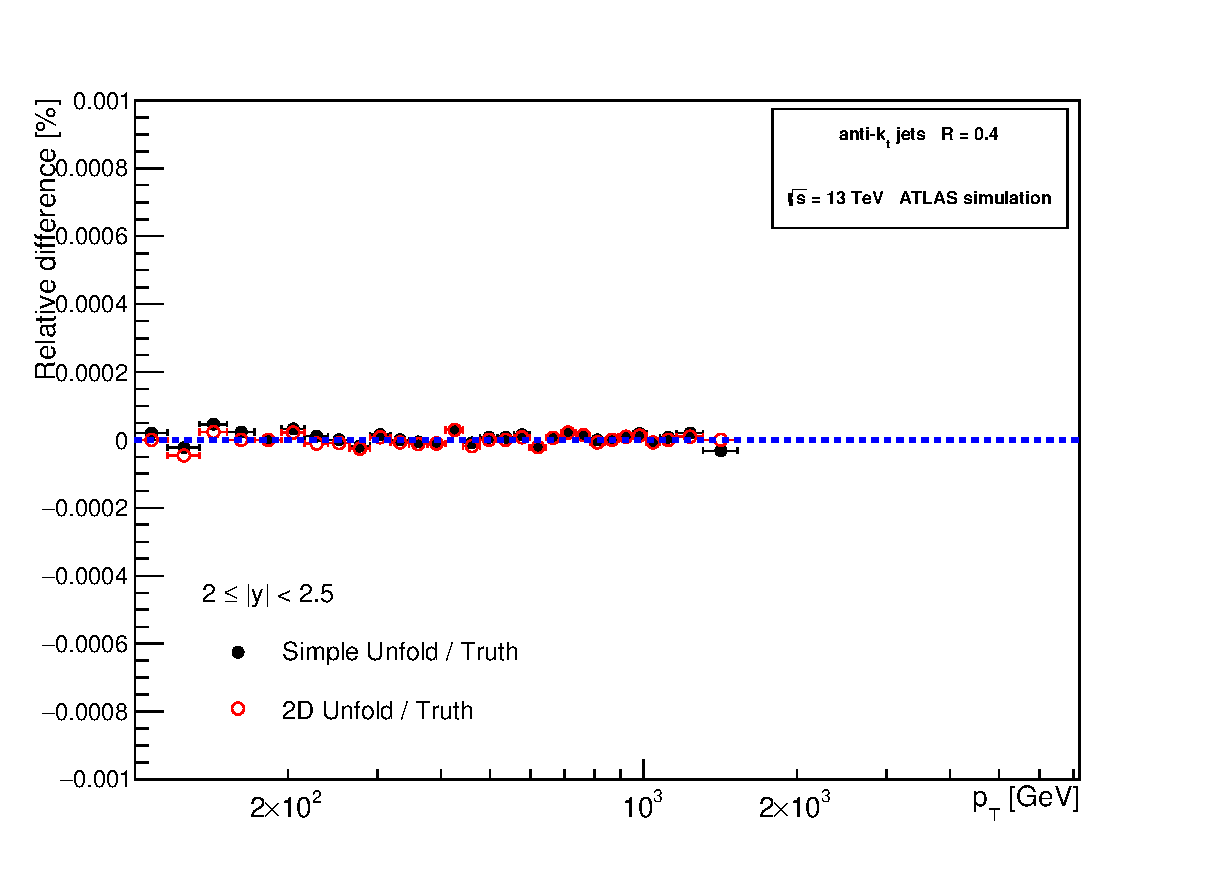
\includegraphics[width=0.49\textwidth]{{Chapter3/UnfoldedSimpleComplex_VS_Truth|abs(y)|2-2.5Compare}.eps}
  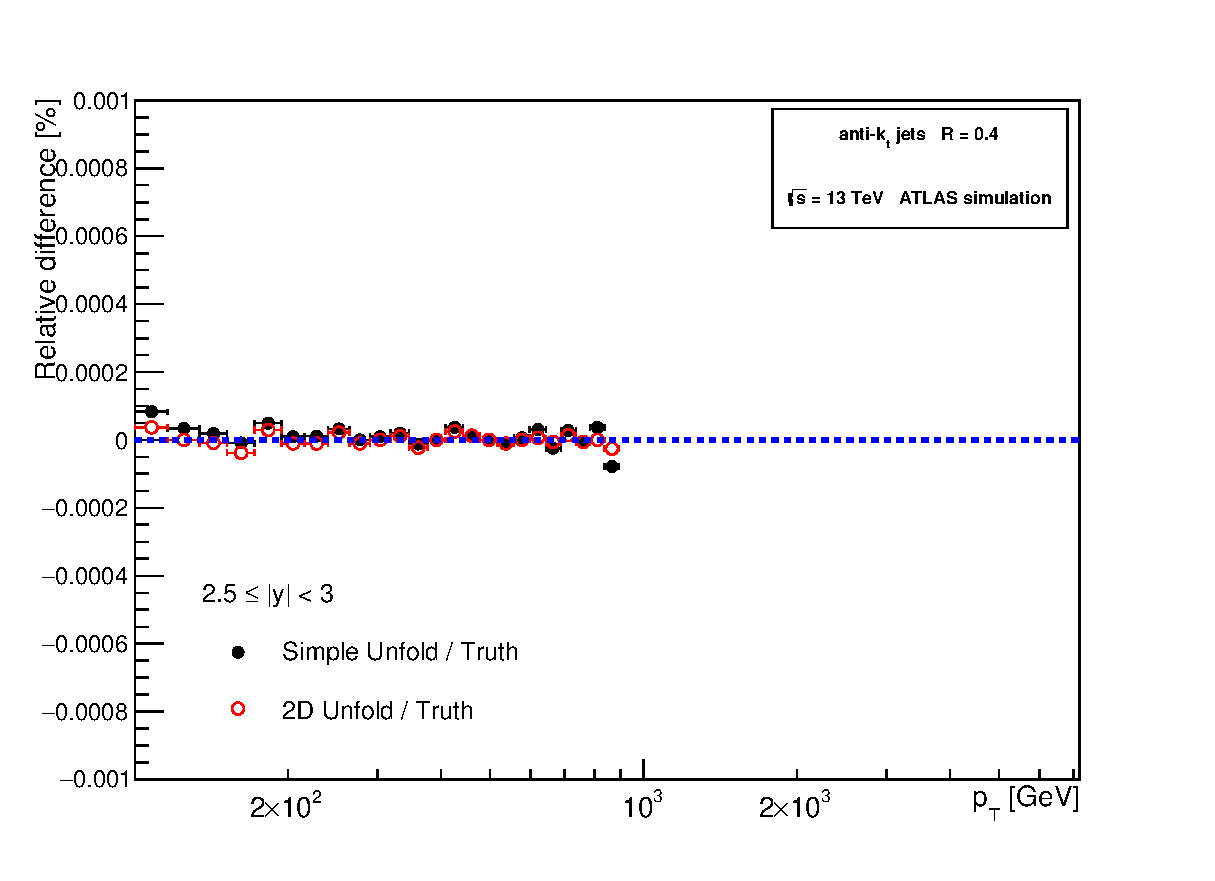
\includegraphics[width=0.49\textwidth]{{Chapter3/UnfoldedSimpleComplex_VS_Truth|abs(y)|2.5-3Compare}.eps}
  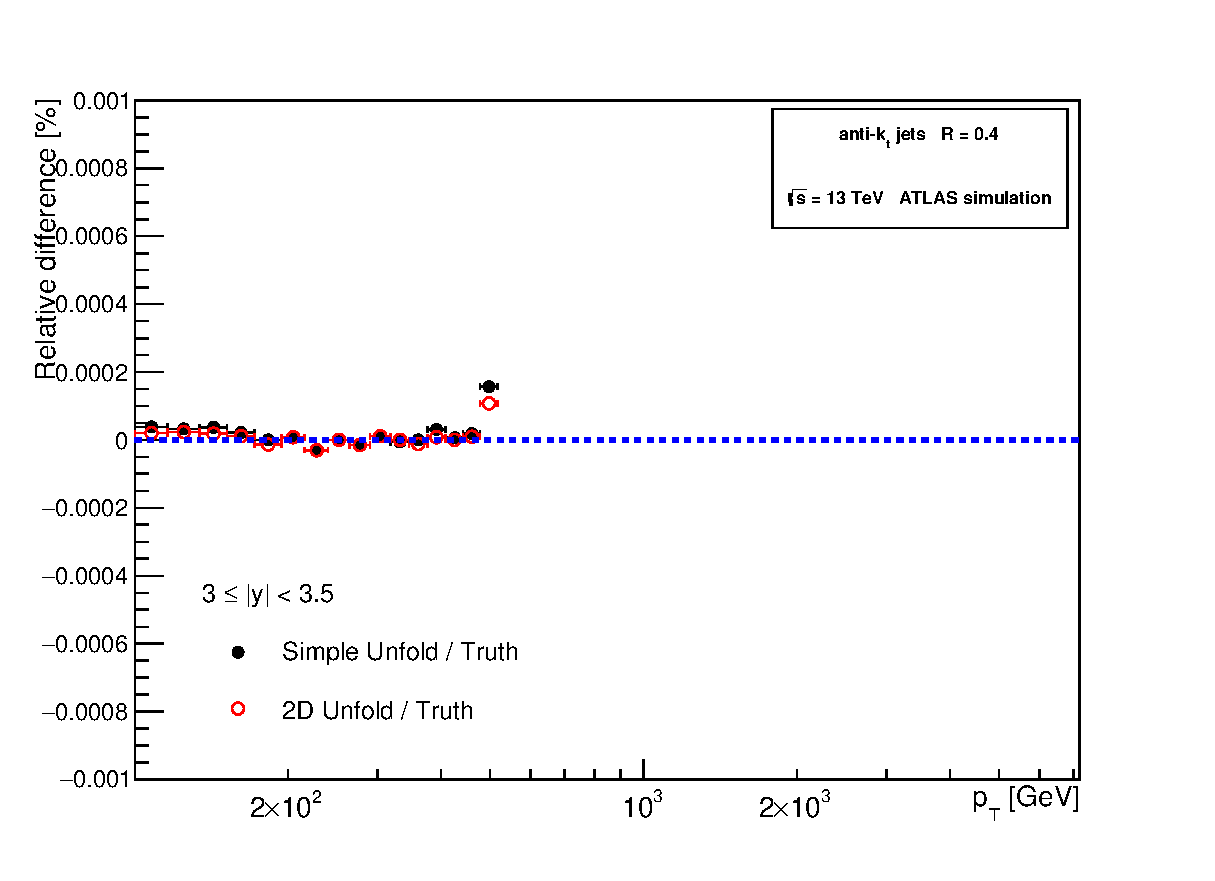
\includegraphics[width=0.49\textwidth]{{Chapter3/UnfoldedSimpleComplex_VS_Truth|abs(y)|3-3.5Compare}.eps}
  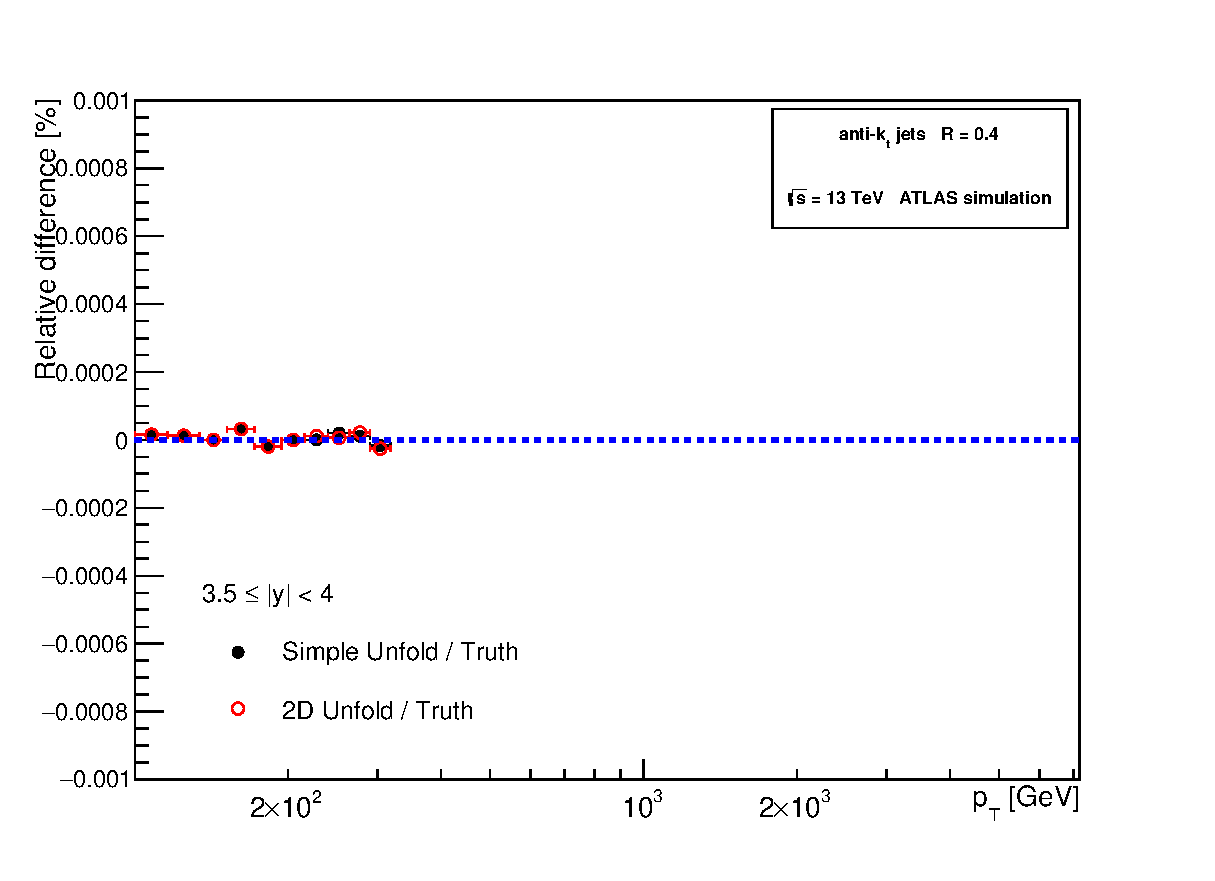
\includegraphics[width=0.49\textwidth]{{Chapter3/UnfoldedSimpleComplex_VS_Truth|abs(y)|3.5-4Compare}.eps}
\end{figure}



\chapter{NLO QCD Prediction}
\label{App:UnfoldingAndPrediction}

\section{Predictions for Run I and Run II}

\begin{center}
\begin{figure}[H]
  \centering
  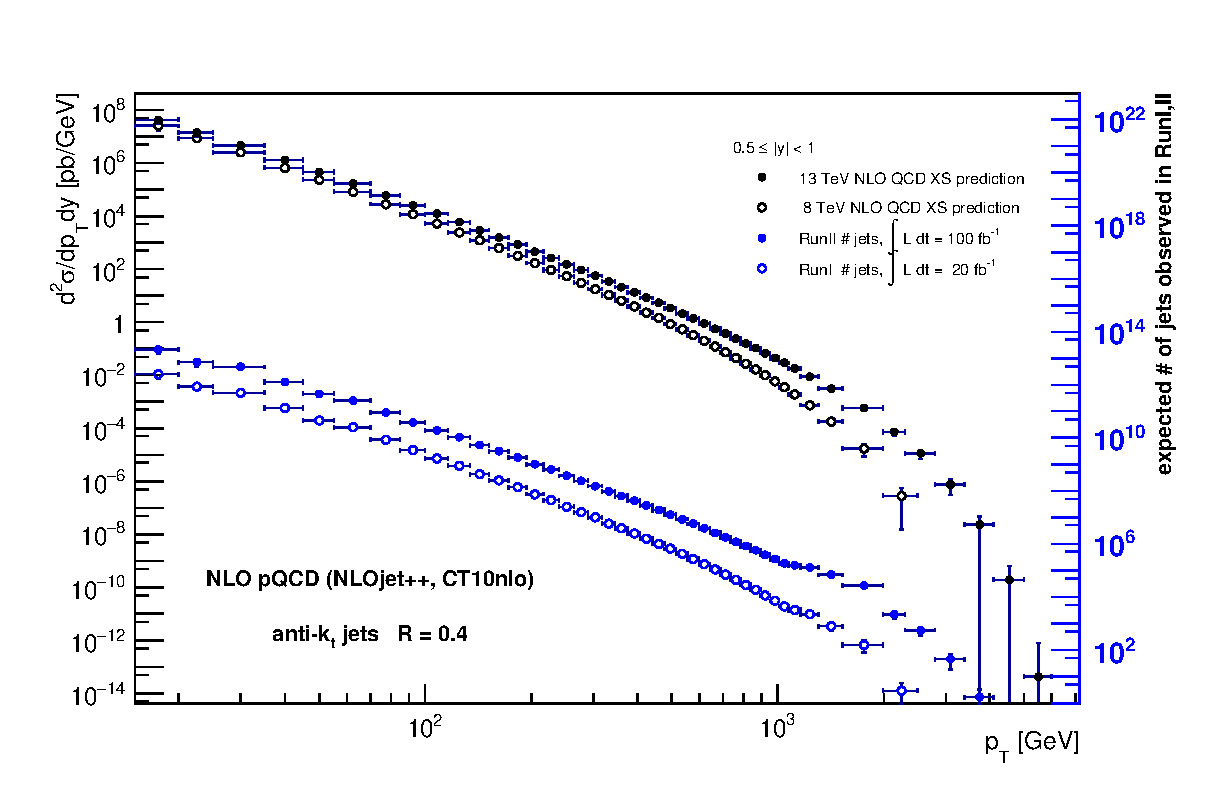
\includegraphics[width=0.8\textwidth]{{Chapter3/PredictionCompare1}.eps}
\end{figure}
\end{center}

\begin{figure}[p]
  \centering
  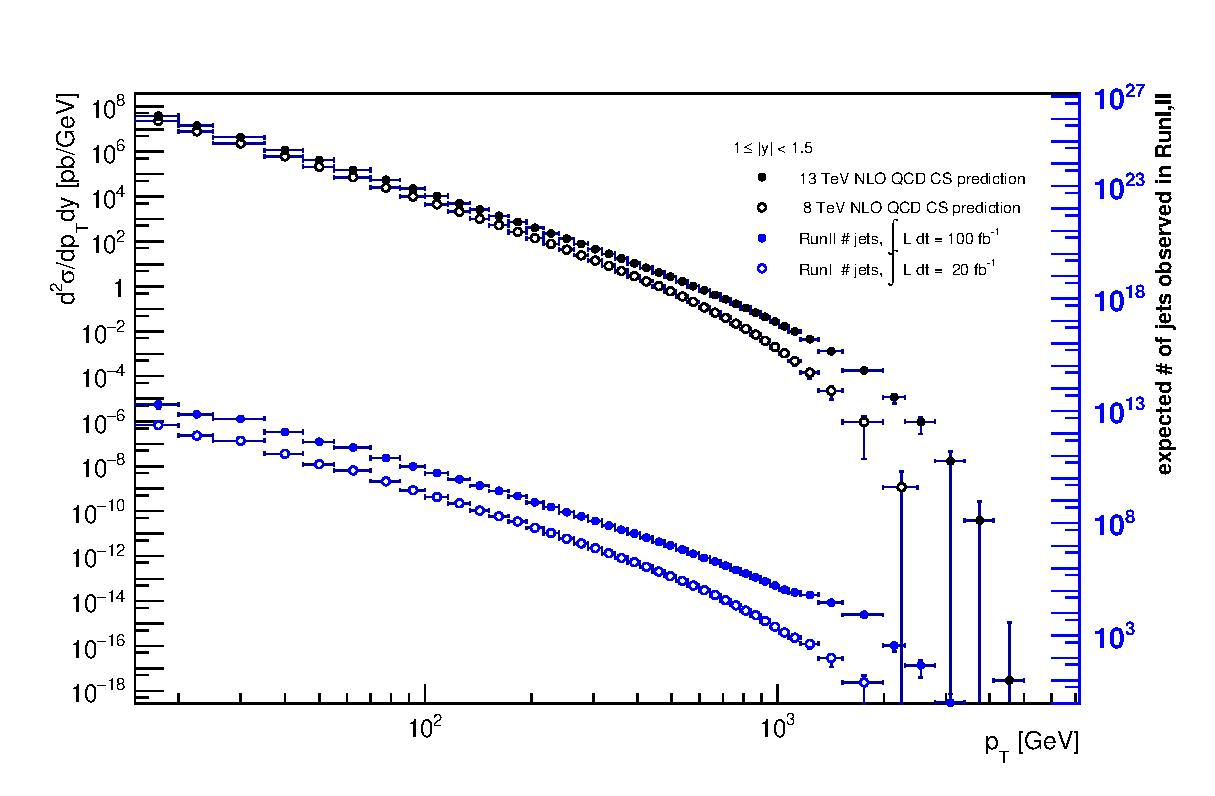
\includegraphics[width=0.8\textwidth]{{Chapter3/PredictionCompare2}.eps}
  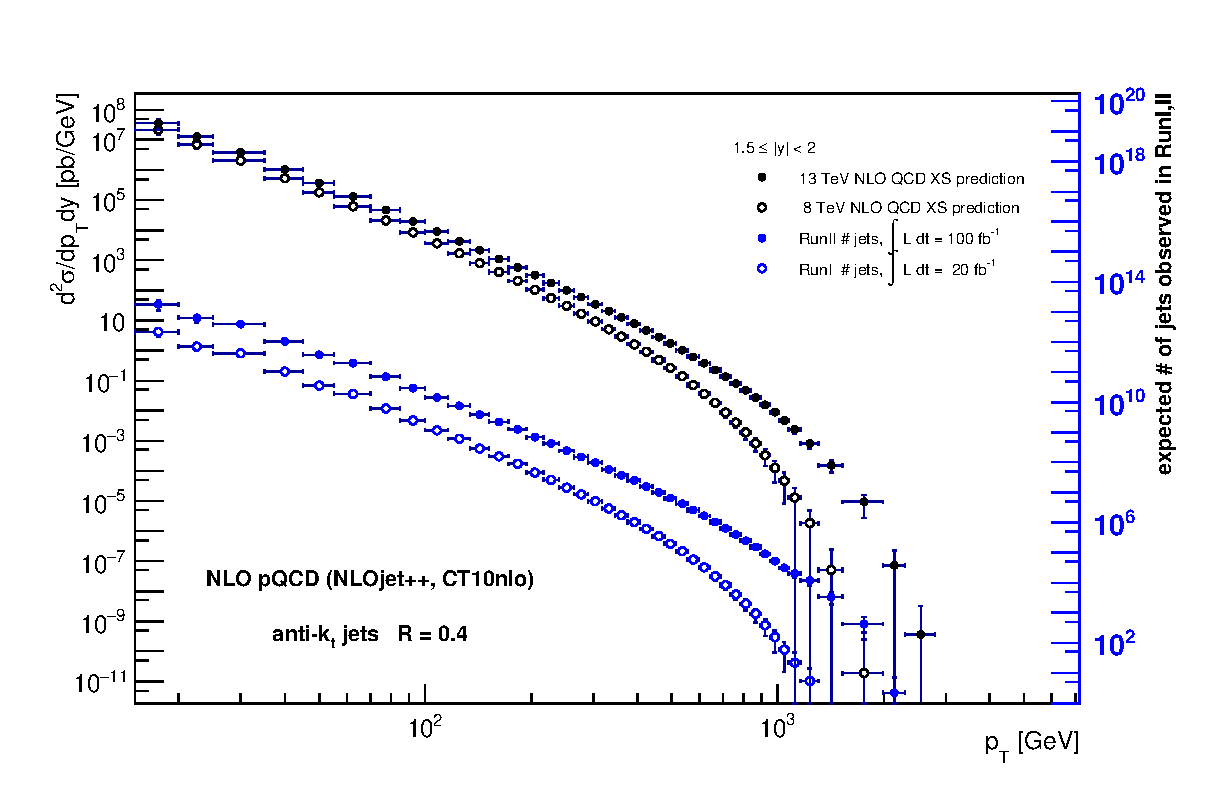
\includegraphics[width=0.8\textwidth]{{Chapter3/PredictionCompare3}.eps}
\end{figure}

\begin{figure}[p]
  \centering
  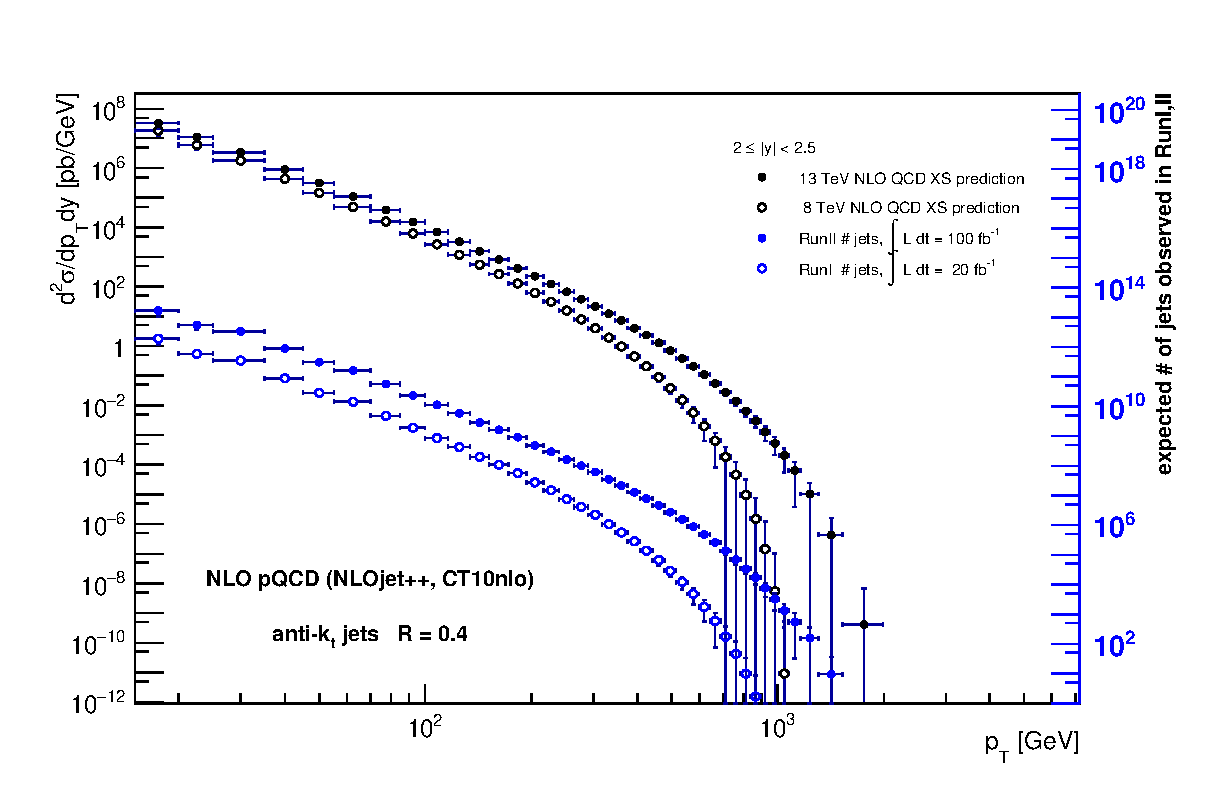
\includegraphics[width=0.8\textwidth]{{Chapter3/PredictionCompare4}.eps}
  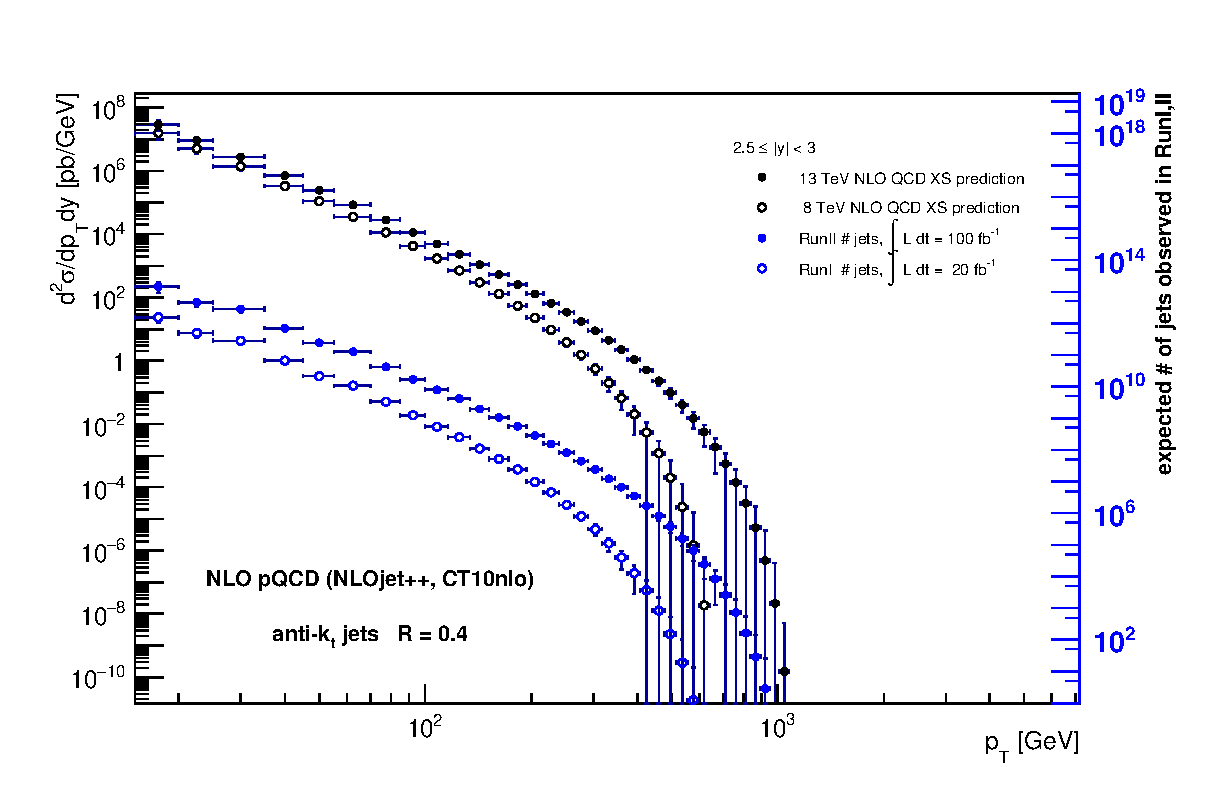
\includegraphics[width=0.8\textwidth]{{Chapter3/PredictionCompare5}.eps}
\end{figure}

\section{NLO Uncertainties}

\begin{center}
\begin{figure}[H]
  \centering
  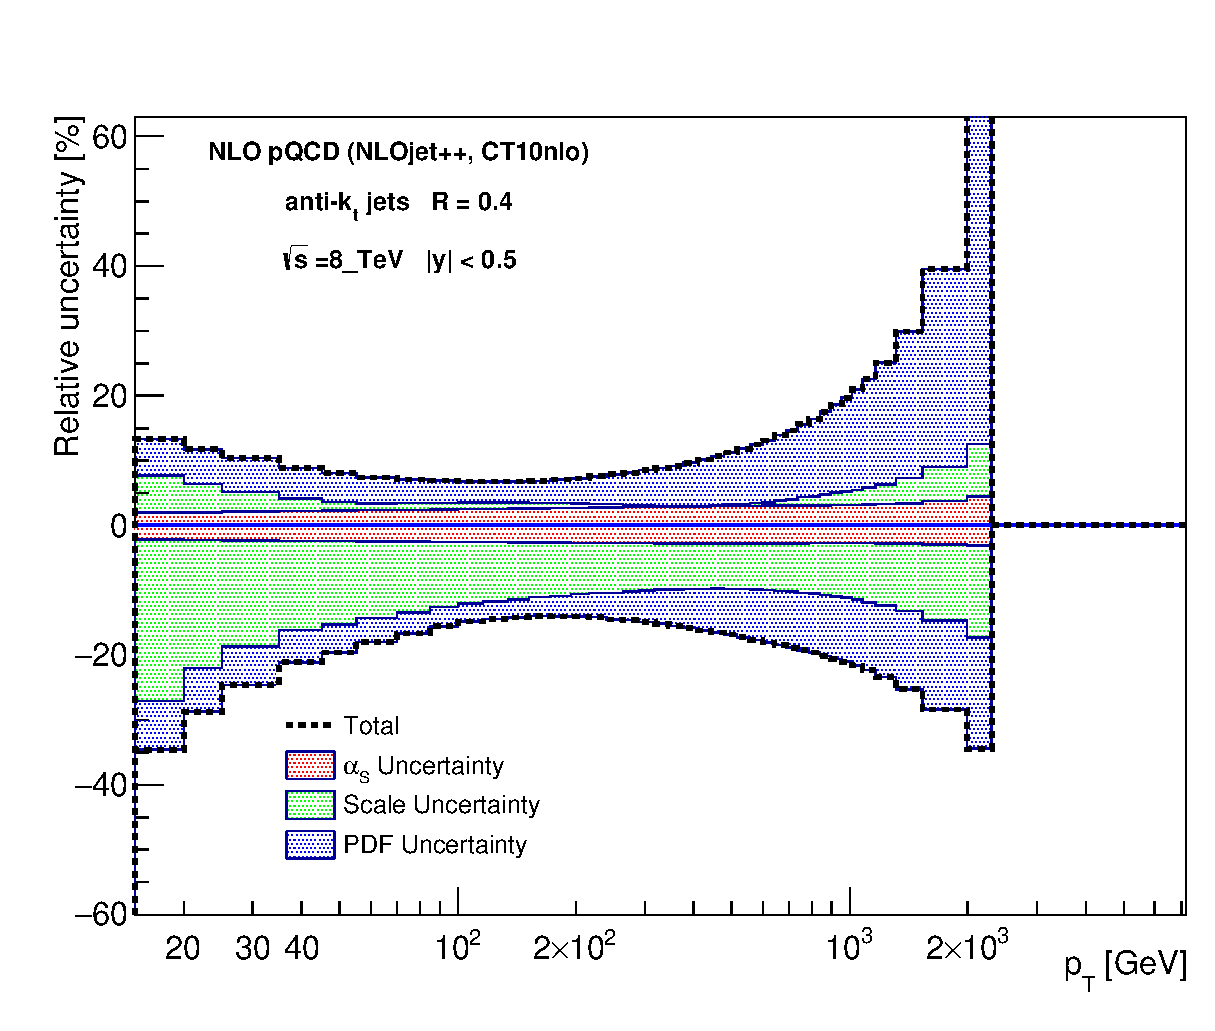
\includegraphics[width=0.49\textwidth]{{Chapter3/NLO_Systematics8_TeV0}.eps}
  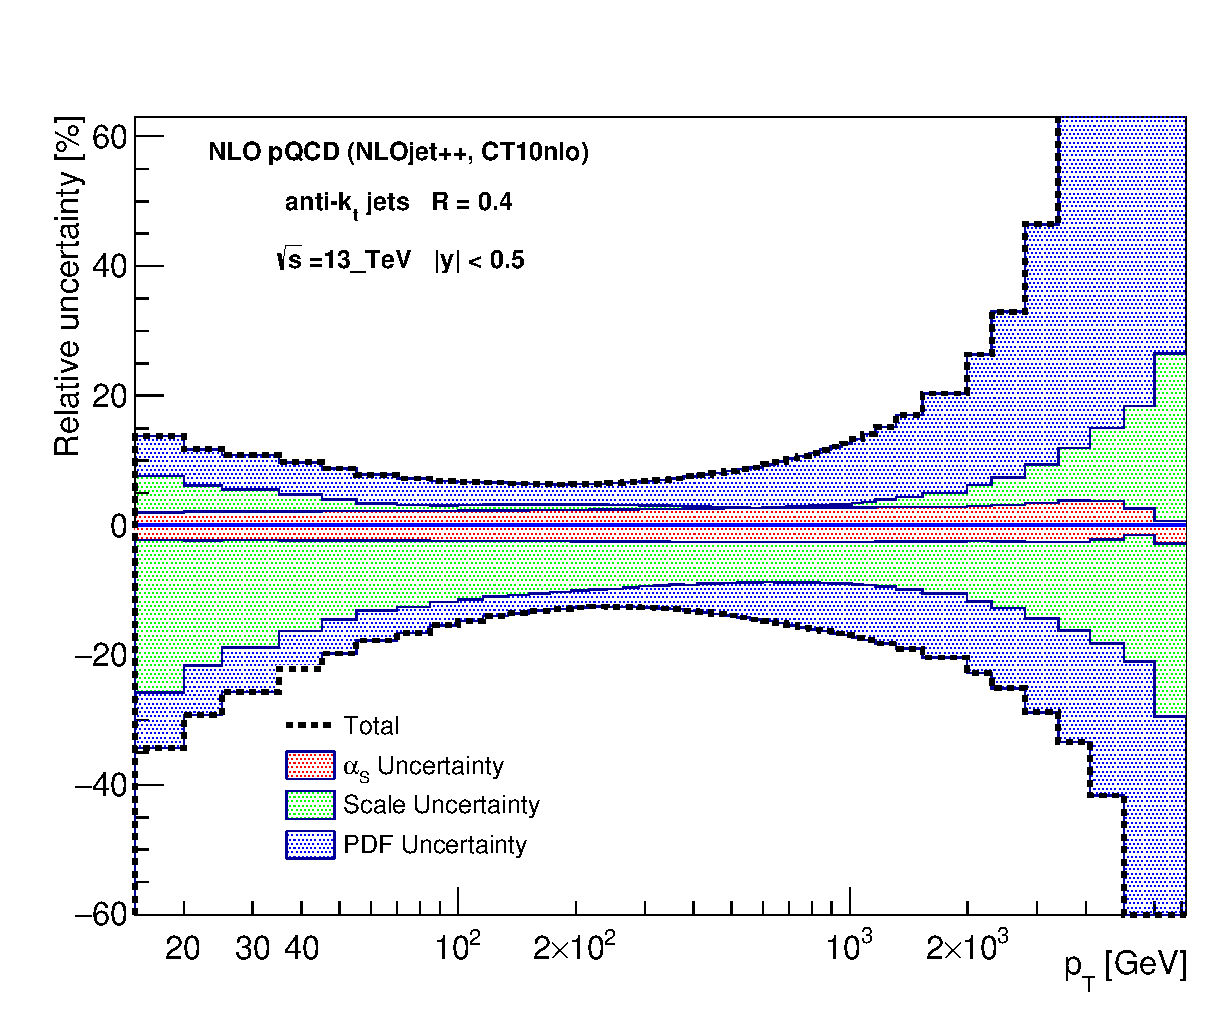
\includegraphics[width=0.49\textwidth]{{Chapter3/NLO_Systematics13_TeV0}.eps}
  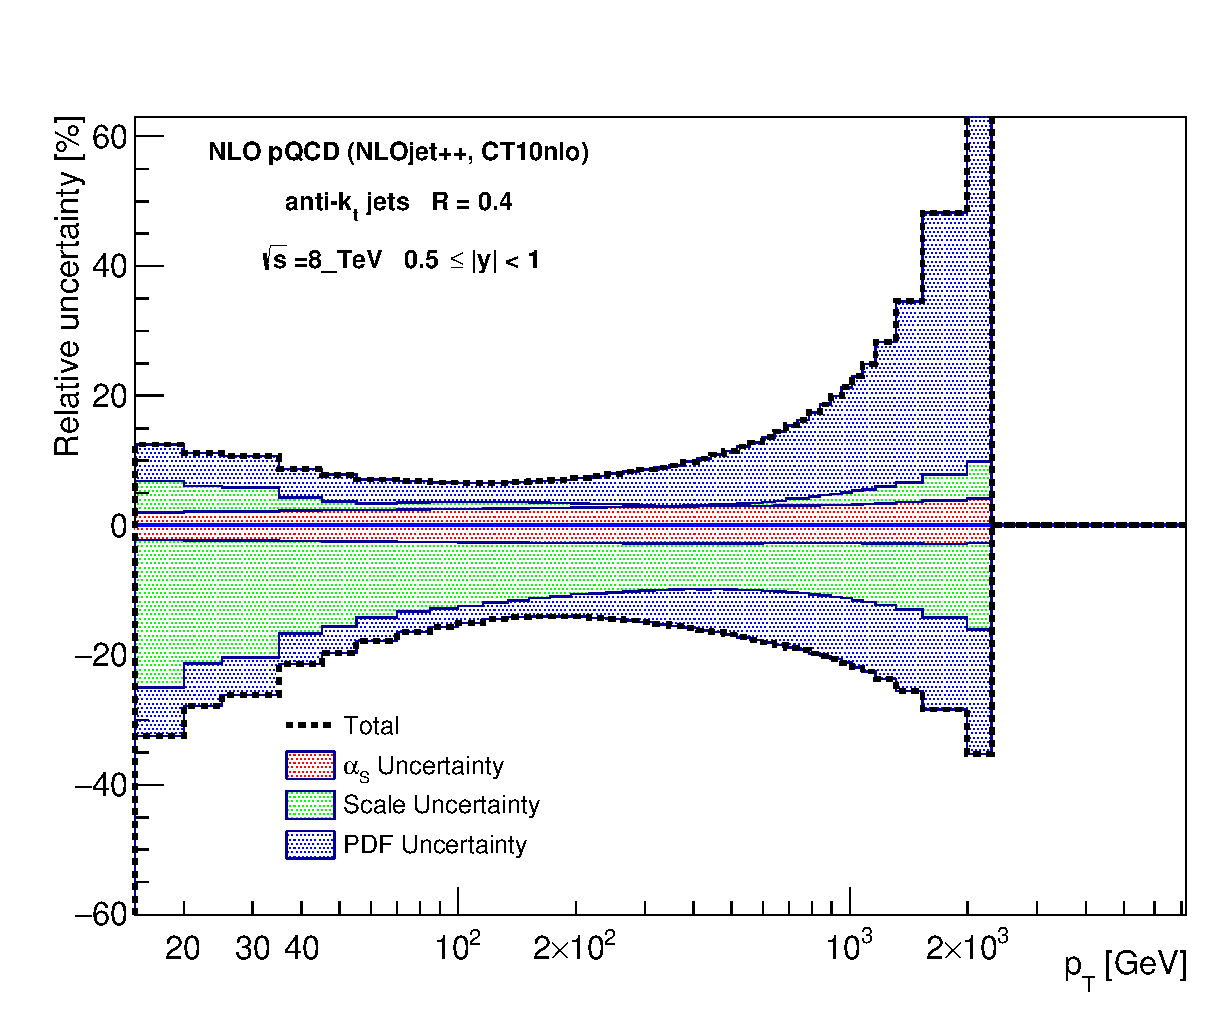
\includegraphics[width=0.49\textwidth]{{Chapter3/NLO_Systematics8_TeV1}.eps}
  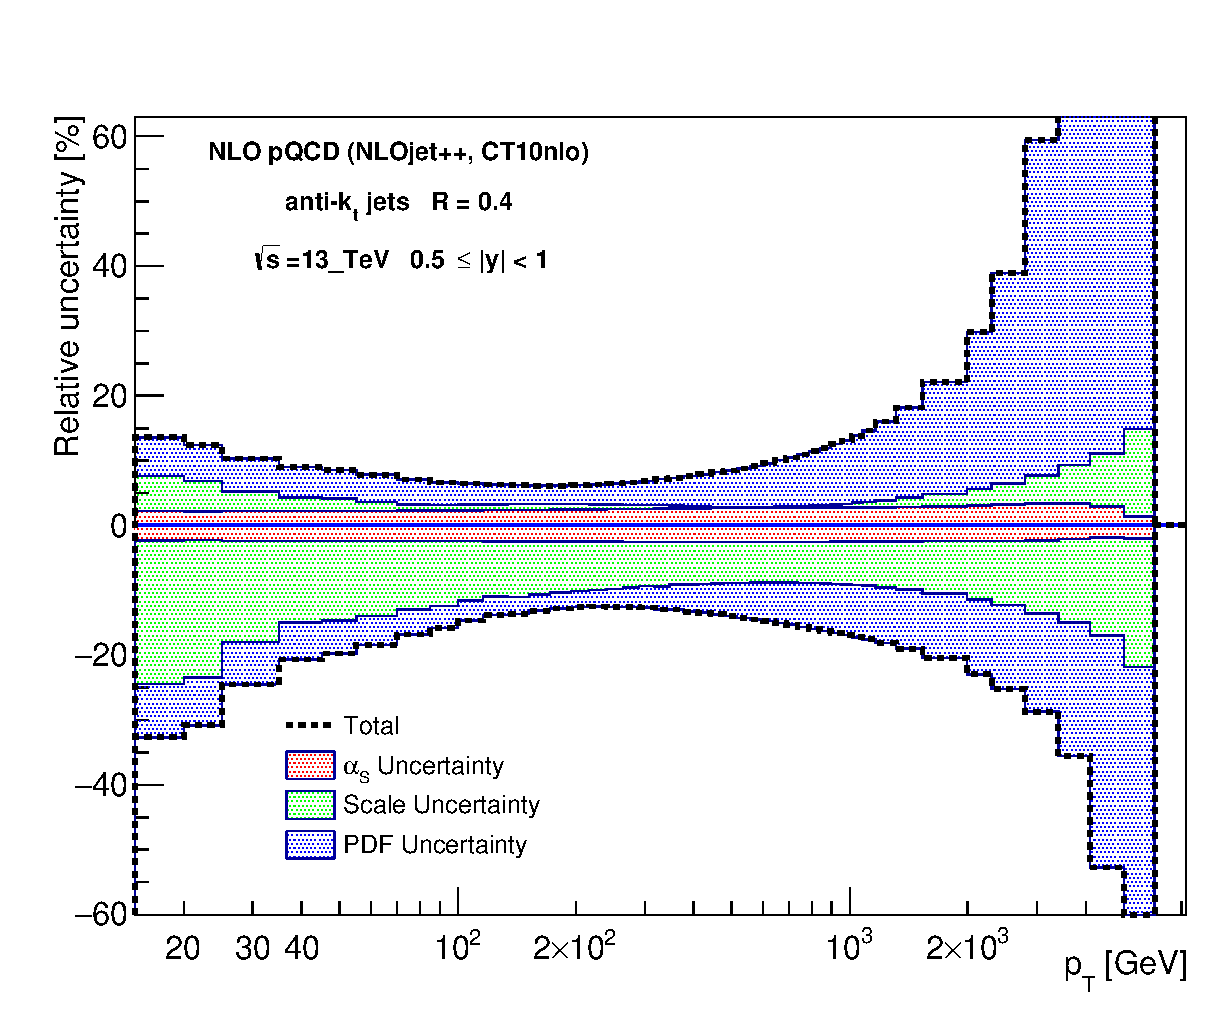
\includegraphics[width=0.49\textwidth]{{Chapter3/NLO_Systematics13_TeV1}.eps}
  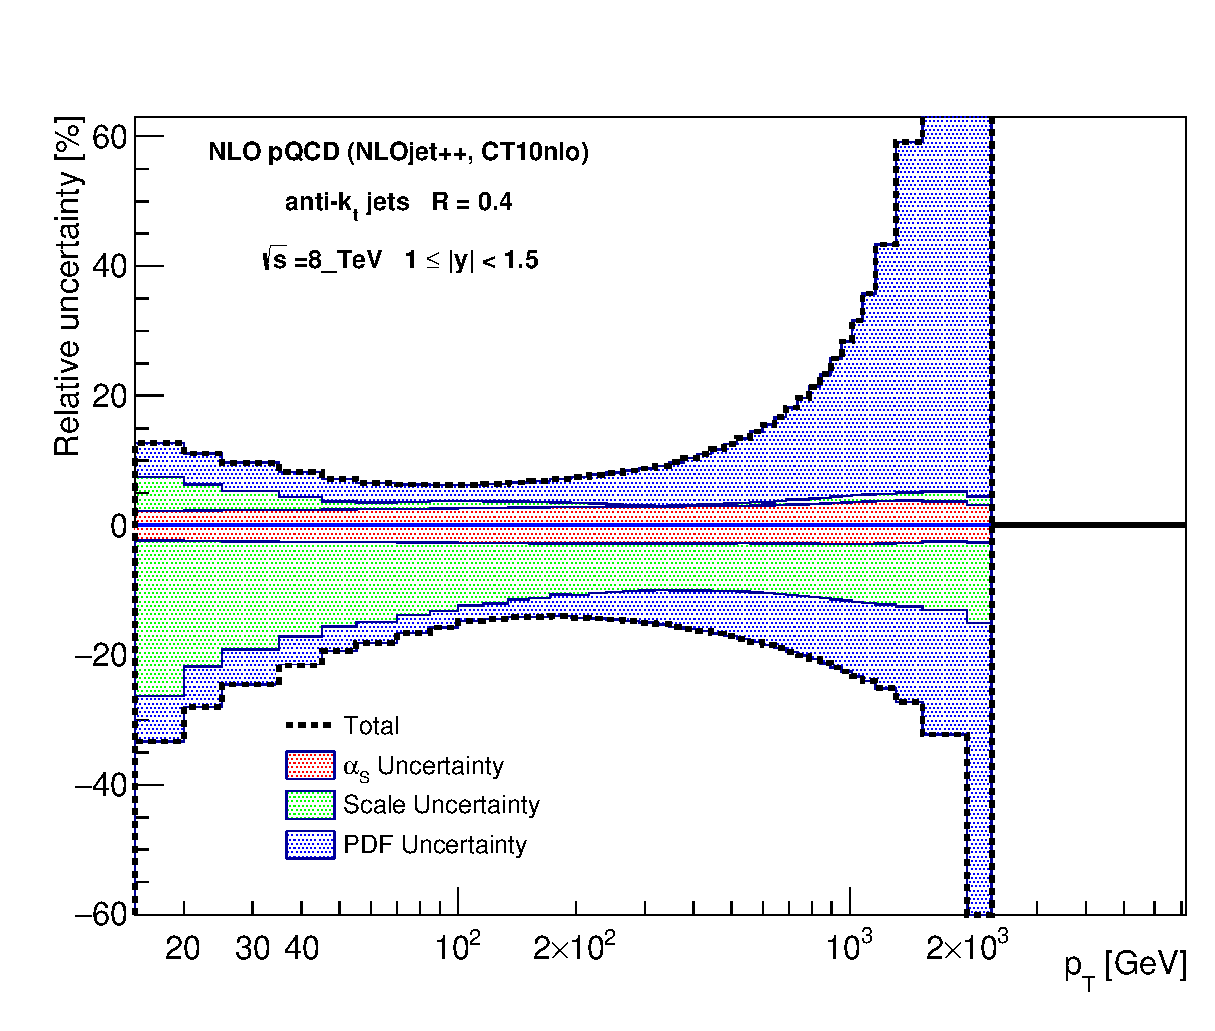
\includegraphics[width=0.49\textwidth]{{Chapter3/NLO_Systematics8_TeV2}.eps}
  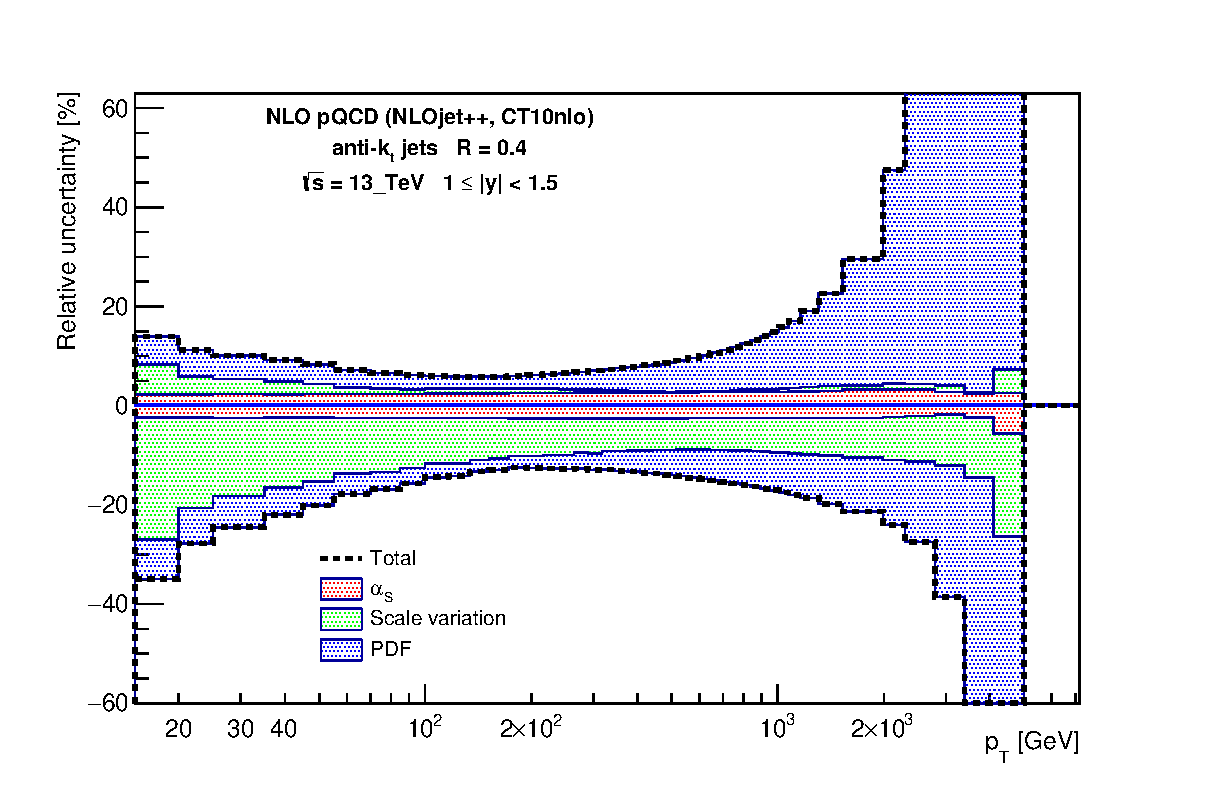
\includegraphics[width=0.49\textwidth]{{Chapter3/NLO_Systematics13_TeV2}.eps}
\end{figure}
\end{center}

\begin{figure}[p]
  \centering
  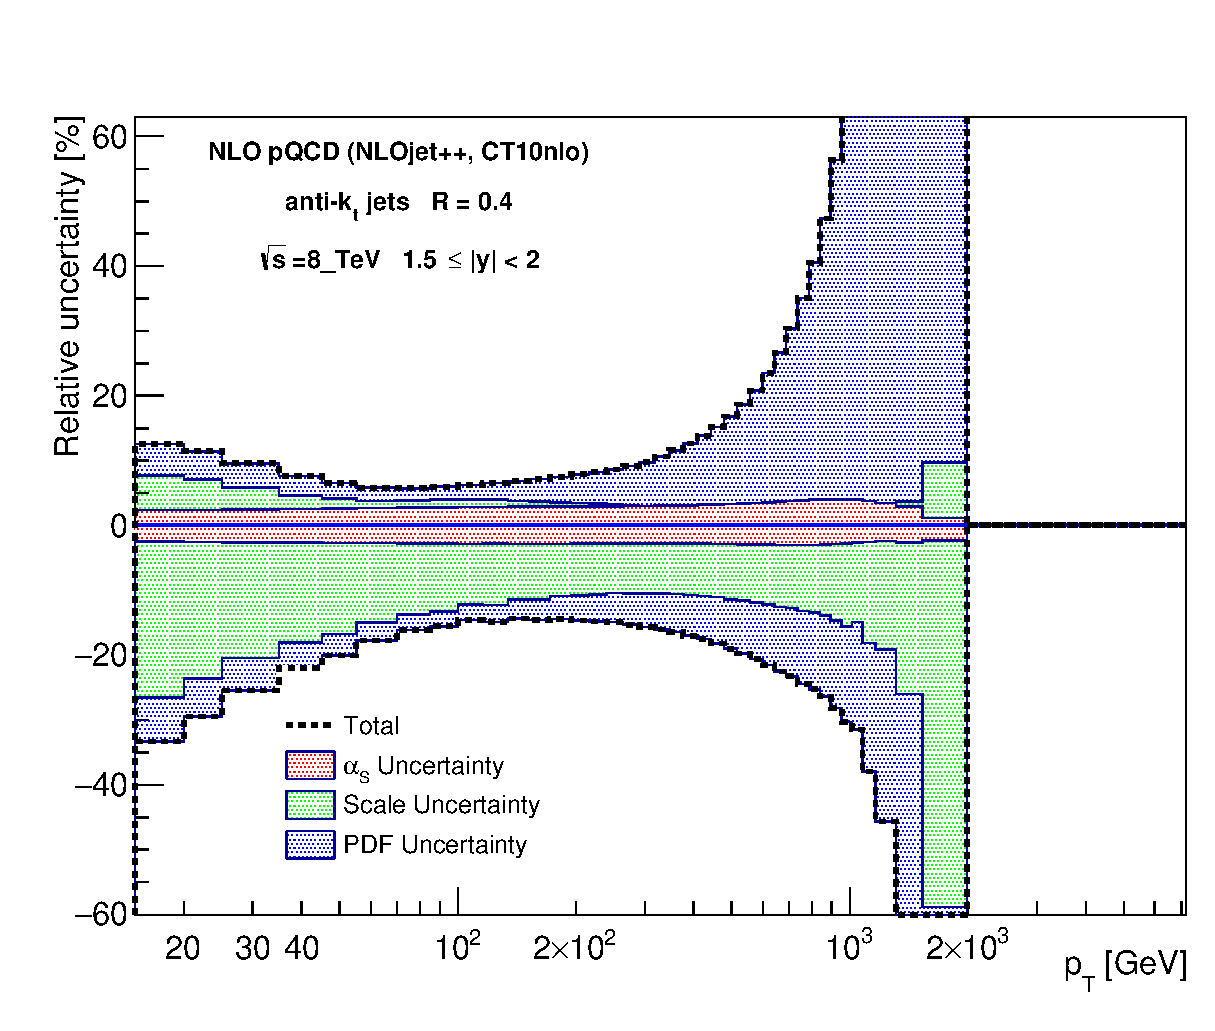
\includegraphics[width=0.49\textwidth]{{Chapter3/NLO_Systematics8_TeV3}.eps}
  \includegraphics[width=0.49\textwidth]{{Chapter3/NLO_Systematics13_TeV3}.eps}
  \includegraphics[width=0.49\textwidth]{{Chapter3/NLO_Systematics8_TeV4}.eps}
  \includegraphics[width=0.49\textwidth]{{Chapter3/NLO_Systematics13_TeV4}.eps}
  \includegraphics[width=0.49\textwidth]{{Chapter3/NLO_Systematics8_TeV5}.eps}
  \includegraphics[width=0.49\textwidth]{{Chapter3/NLO_Systematics13_TeV5}.eps}
\end{figure}

\section{Pythia and NLO}

\begin{center}
\begin{figure}[H]
  \centering
  \includegraphics[width=0.49\textwidth]{{Chapter3/Truth_VS_Prediction|abs(y)|0-0.5Compare}.eps}
  \includegraphics[width=0.49\textwidth]{{Chapter3/Truth_VS_Prediction|abs(y)|0.5-1Compare}.eps}
  \includegraphics[width=0.49\textwidth]{{Chapter3/Truth_VS_Prediction|abs(y)|1-1.5Compare}.eps}
  \includegraphics[width=0.49\textwidth]{{Chapter3/Truth_VS_Prediction|abs(y)|1.5-2Compare}.eps}
  \includegraphics[width=0.49\textwidth]{{Chapter3/Truth_VS_Prediction|abs(y)|2-2.5Compare}.eps}
  \includegraphics[width=0.49\textwidth]{{Chapter3/Truth_VS_Prediction|abs(y)|2.5-3Compare}.eps}
\end{figure}
\end{center}

\end{appendices}
